\documentclass[pdflatex,sn-basic]{sn-jnl}

\usepackage{graphicx}
\usepackage{booktabs}
\usepackage{amsmath}
\usepackage{float}
\usepackage{subcaption}
\usepackage{xurl}

\begin{document}

\title[Accuracy Without Profit]{Accuracy Without Profit: A Statistical Evaluation of Machine Learning Profitability in the English Premier League}

\author*[1]{\fnm{Mostafa} \sur{Shams} (Corresponding author, ORCID: \url{https://orcid.org/0009-0001-8852-193X})}\email{mustafa.samy2022385@ci.menofia.edu.eg}
\affil*[1]{\orgdiv{Faculty of Computer and Information}, \orgname{Menoufia University}, \country{Egypt}}

\abstract{This study explores why highly accurate machine learning models still lose money in the English Premier League betting market (2000–2021, $N=9,935$ matches). Using a strict Walk-Forward Validation approach to prevent look-ahead bias, we tested tree-based algorithms (XGBoost, LightGBM, Random Forest) alongside a simple Logistic Regression baseline. We found a clear disconnect between accuracy and profit: for example, Logistic Regression achieved the highest accuracy (54.1\%) but suffered the worst financial loss (-2.89\% ROI). Our analysis traces this failure to three main factors: (1) \textbf{Alpha Decay}, where the models' profitable edge slowly vanished after 2015 as bookmakers became more efficient; (2) \textbf{COVID-19 Concept Drift}, where the historical home-field advantage dropped from 46.5\% to 42.5\% in empty stadiums during 2020, severely tricking the models; and (3) \textbf{Calibration Error}, where severe overconfidence (ECE $\approx$ 0.145) caused mathematical risk-management strategies like the Kelly Criterion to lose 73\% of a starting bankroll. 

Crucially, we uncover a "Market Surrender Paradox": mathematically fixing the model's overconfidence using Isotonic Regression perfectly corrects the error (dropping ECE to 0.028), but this simply forces the model to agree with the bookmaker, guaranteeing a loss on flat bets due to the bookmaker's built-in fee. However, when we pair these properly calibrated probabilities with a highly cautious 10\% Fractional Kelly strategy, the exact same model transforms a 73\% bankroll loss into a stable 6\% long-term profit. Ultimately, this research proves that in efficient betting markets, chasing raw accuracy is a trap; long-term survival requires both honest probability calibration and strict bankroll management.

\vspace{0.4em}
\noindent \textbf{Reproducibility:} All code, datasets, and full statistical reports generated during this study are publicly available for review and replication at: \url{https://github.com/MostafaShams5/Research-Accuracy-Without-Profit}.}

\keywords{Machine Learning, Sports Economics, Probability Calibration, Kelly Criterion, Adaptive Markets Hypothesis, Concept Drift}

\maketitle
\section{Introduction}

Predicting the future is the central goal of data science. However, not all datasets are created equal. Some are static, waiting to be solved, while others are "adversarial"—meaning there is an opponent on the other side actively trying to prevent correct prediction. Sports betting provides a laboratory for studying these adversarial environments. Unlike the stock market, which acts as a continuous flow of prices, a sports match has a definite start and end. The "price" (the odds) is set by bookmakers who are highly motivated to be accurate. If a predictive model can consistently beat these odds, it proves that the market has a leak—an inefficiency that can be exploited. Conversely, if a sophisticated model cannot make a profit, it suggests the market has become "efficient," meaning the price already reflects all available information.

This paper investigates the evolution of this efficiency. While early research often found small cracks in the bookmakers' armor, we ask: "How has the market learned to beat machine learning?"

To answer this, we applied tree-based machine learning architectures (XGBoost, LightGBM, Random Forest) alongside a Logistic Regression baseline to twenty-one years of English Premier League football data (2000–2021). Our approach was strictly historical. We did not let the models "peek" at the future; we trained them season by season using Walk-Forward Validation, simulating exactly what a data scientist would have experienced in real time.

The results challenge the idea of a sudden structural break in market efficiency. We found that while algorithms form their own distinct "opinion" from the bookmaker's odds, they struggle to generate long-term profit. Our analysis reveals a clear timeline of Alpha Decay: strategies that generated reliable profits in the mid-2000s slowly degraded as bookmakers became increasingly sophisticated, with the edge largely evaporating after 2015. We also identify a critical real-world vulnerability in predictive modeling: when stadiums emptied during the 2020 COVID-19 pandemic, the historical home-field advantage vanished overnight, causing severe concept drift that tricked the models.

Most importantly, we isolate a fundamental flaw in how these models operate: while they achieve high accuracy, they are dangerously overconfident. This gap between confidence and reality—calibration error—destroys standard mathematical betting strategies like the Kelly Criterion. We demonstrate a profound "Market Surrender Paradox": if you mathematically fix this overconfidence using post-hoc calibration, the model simply learns to copy the bookmaker, guaranteeing a financial loss due to the bookmaker's built-in margin. However, by combining properly calibrated probabilities with a highly cautious fractional staking strategy, we transform a massive bankruptcy loss into a stable profit. This proves that in adversarial markets, maximizing raw accuracy is a trap; survival depends entirely on strict probability calibration and rigorous bankroll management.

% --- RELATED WORK ---
\section{Related Work and Background}

Before detailing our experiments, it is necessary to contextualize our findings within the broader literature of sports economics and statistical modeling. While the application of modern Machine Learning to sports betting is a relatively new field, it rests on two well-established pillars of research: the economic theory of Efficient Markets and the statistical problem of Probability Calibration.

\subsection{The Efficient Market and the Strategic Bookmaker}
The primary obstacle to profitable prediction is the Efficient Market Hypothesis (EMH). Originally proposed for financial markets, the theory suggests that asset prices already contain all known information, making consistent profit impossible without inside information \cite{fama1970}. In the specific context of sports, Sauer (1998) refined this into the "Efficient Forecast Hypothesis," arguing that wagering markets are efficient if the closing odds are unbiased predictors of match outcomes \cite{sauer1998}.

However, sports betting markets differ from financial markets in one critical way: the presence of an active opponent. Levitt (2004) argues that bookmakers are not merely passive market-makers but "adversarial agents." They are highly skilled at setting prices that not only reflect true probabilities but also exploit human biases—such as the "favorite-longshot bias"—to maximize their own profit while minimizing risk \cite{levitt2004, griffith1949}. This creates a strategic environment where a predictive model is not just solving a math problem, but battling an optimized pricing algorithm.

To understand how these markets evolve over time, we look to Lo's (2004) Adaptive Markets Hypothesis (AMH) \cite{lo2004}. The AMH posits that market efficiency is not a fixed, binary state, but a dynamic, evolutionary process. As new predictive models (such as machine learning) discover temporary inefficiencies, market-makers adapt their own pricing algorithms to eliminate them, causing the profitable edge to decay over time. As our study aims to demonstrate through formal structural break testing, the gap between "market efficiency" and "model accuracy" has closed significantly in the big-data era through exactly this type of evolutionary alpha decay.

\subsection{From Statistical History to Calibration Errors}
To beat these efficient markets, researchers initially relied on parametric statistical models. The foundational work by Dixon and Coles (1997) established that simple averages are insufficient; models must account for time-decay, weighting recent match results more heavily than older ones \cite{dixon1997}. This concept of "recent form" remains a standard feature in modern engineering, including our own.

As the field moved from statistical models to Machine Learning (e.g., Random Forests and Gradient Boosting), the primary evaluation metric shifted heavily toward raw Accuracy. However, recent literature argues that in adversarial betting environments, Accuracy is a deeply misleading metric. The foundational framework for this was established by Murphy and Winkler (1987), who introduced the distributions-oriented approach to probability forecasting. They proved that evaluating a forecast requires separating its "resolution" (accuracy) from its "reliability" (calibration) \cite{murphy1987}. Building on this, Wheatcroft (2020) demonstrated that a sports betting strategy's profitability is far more sensitive to calibration error than to raw predictive accuracy \cite{wheatcroft2019}. This is why it is critical to benchmark complex, opaque algorithms against principled generalized linear models (like Logistic Regression), which naturally produce well-calibrated probabilities.

This distinction is critical. If a model predicts a 60\% probability of a win, but the event occurs only 50\% of the time, the model is inherently "miscalibrated" \cite{guo2017}. Walsh and Joshi (2024) recently confirmed that when using aggressive risk-management strategies like the Kelly Criterion \cite{kelly1956}, calibration-optimized models significantly outperform accuracy-optimized ones \cite{walsh2024}. To mitigate the severe penalty of overconfidence, financial mathematics literature strongly advocates for the "Fractional Kelly" approach. As detailed by MacLean, Thorp, and Ziemba (2010), betting a fixed fraction (e.g., 10\%) of the Kelly optimal stake provides a critical margin of safety against parameter uncertainty, drastically reducing bankroll volatility \cite{maclean2010}. Our paper extends this literature by proving that applying post-hoc isotonic calibration combined with a Fractional Kelly strategy is the mathematical prerequisite for surviving the modern bookmaker's margin.


\section{Methodology and Data}

To ensure our results were robust, we utilized a testing method that strictly followed the flow of time, preventing the common mistake of using future data to predict the past.

\subsection{The Dataset: English Premier League (2000–2021)}
Our primary dataset covers twenty-one seasons of English top-flight football \cite{kaggleEPL}. The dataset comprises exactly $N = 9,935$ professional matches.

To establish a baseline for our models, it is critical to understand the natural distribution of match outcomes. Over our 21-season sample, the results are strongly skewed by the structural home-field advantage of the sport: Home Wins ($H$) account for 46.88\% of all matches, Away Wins ($A$) account for 28.42\%, and Draws ($D$) account for 24.69\%. Any successful machine learning model must learn to predict beyond this basic historical skew.

To create a consistent input for the models, we performed the following preprocessing steps:
\begin{enumerate}
    \item \textbf{Market Consensus (Odds):} We utilized the average odds across all available major bookmakers for Home Win, Draw, and Away Win. This ensures the model is training on the global market opinion rather than a single provider's price.
    \item \textbf{Team Fundamentals (Feature Engineering):} We engineered rolling window features representing each team's form over the Last 5 Games (L5). Specifically, we computed L5 averages for Points, Goals Conceded, Shots, Shots on Target, and Corners. This transforms raw match results into trend metrics.
\end{enumerate}

\begin{table}[htbp]
\centering
\caption{Snapshot of Transformed Input Data (First 10 Rows)}
\label{tab:data_snapshot}
\setlength{\tabcolsep}{1.5pt}
\scriptsize
\begin{tabular}{@{}lllc|ccc|ccccc|ccccc@{}}
\toprule
\textbf{Date} & \textbf{Home} & \textbf{Away} & \textbf{FTR} & \textbf{HO} & \textbf{DO} & \textbf{AO} & \textbf{H\_Pts} & \textbf{H\_GC} & \textbf{H\_S} & \textbf{H\_ST} & \textbf{H\_C} & \textbf{A\_Pts} & \textbf{A\_GC} & \textbf{A\_S} & \textbf{A\_ST} & \textbf{A\_C} \\ \midrule
2001-08-20 & Everton & Tottenham & D & 2.25 & 3.20 & 2.75 & 3.0 & 1.0 & 12.0 & 9.0 & 4.0 & 1.0 & 0.0 & 8.0 & 2.0 & 6.0 \\
2001-08-21 & Ipswich & Derby & H & 1.66 & 3.30 & 4.50 & 0.0 & 1.0 & 10.0 & 4.0 & 1.0 & 3.0 & 1.0 & 7.0 & 3.0 & 4.0 \\
2001-08-21 & Bolton & Middlesbr. & H & 2.20 & 3.25 & 2.75 & 3.0 & 0.0 & 18.0 & 8.0 & 5.0 & 0.0 & 4.0 & 6.0 & 2.0 & 2.0 \\
2001-08-21 & Arsenal & Leeds & A & 1.72 & 3.25 & 4.20 & 3.0 & 0.0 & 14.0 & 9.0 & 6.0 & 3.0 & 0.0 & 16.0 & 6.0 & 10.0 \\
2001-08-22 & Blackburn & Man Utd & D & 4.50 & 3.30 & 1.66 & 0.0 & 2.0 & 14.0 & 4.0 & 10.0 & 3.0 & 2.0 & 12.0 & 6.0 & 6.0 \\
2001-08-22 & Fulham & Sunderland & H & 1.90 & 3.20 & 3.50 & 0.0 & 3.0 & 8.0 & 5.0 & 4.0 & 3.0 & 0.0 & 12.0 & 6.0 & 1.0 \\
2001-08-25 & Arsenal & Leicester & H & 1.22 & 5.00 & 9.50 & 1.5 & 1.0 & 14.0 & 7.0 & 8.0 & 0.0 & 5.0 & 6.0 & 1.0 & 3.0 \\
2001-08-25 & Blackburn & Tottenham & H & 2.30 & 3.10 & 2.75 & 0.5 & 2.0 & 13.0 & 4.5 & 6.5 & 1.0 & 0.5 & 7.5 & 2.0 & 3.0 \\
2001-08-25 & Everton & Middlesbr. & H & 2.00 & 3.10 & 3.30 & 2.0 & 1.0 & 15.0 & 10.0 & 6.0 & 0.0 & 2.5 & 8.5 & 3.0 & 2.0 \\
2001-08-25 & Fulham & Derby & D & 1.50 & 3.40 & 6.00 & 1.5 & 1.5 & 10.5 & 5.0 & 6.0 & 1.5 & 2.0 & 4.5 & 2.5 & 3.0 \\ \bottomrule
\end{tabular}%
\vspace{0.5em}
\raggedright
\small{\textit{Note: FTR = Full Time Result. HO/DO/AO = Home/Draw/Away Odds (Averaged). H\_/A\_ = Home/Away Team L5 Rolling Averages. Pts=Points, GC=Goals Conceded, S=Shots, ST=Shots on Target, C=Corners.}}
\end{table}

\subsection{Model Specifications and Ablation}
We treated the sports betting problem as a multi-class classification task with three target classes: Home Win ($H$), Draw ($D$), and Away Win ($A$). To rigorously evaluate the source of the models' predictive power, we conducted an ablation study across three feature subsets: \textbf{Odds-Only} (3 market variables), \textbf{Fundamentals-Only} (10 team metrics), and \textbf{Combined} (13 variables).

We benchmarked four distinct architectures, chosen to span the complexity spectrum from simple linear baselines to advanced tree ensembles:
\begin{itemize}
    \item \textbf{Logistic Regression:} A standard generalized linear model (GLM) utilized as a principled baseline.
    \item \textbf{XGBoost \& LightGBM:} State-of-the-art gradient boosting frameworks trained to minimize multi-class log-loss.
    \item \textbf{Random Forest:} A bagging ensemble of 100 decision trees.
\end{itemize}

Crucially, to test the impact of parameter uncertainty on risk-management strategies, we introduced a fifth variant: \textbf{XGBoost (Calibrated)}. This applies post-hoc Isotonic Regression to the base XGBoost model to mathematically correct its probability distributions. We intentionally abstained from extensive hyperparameter grid-searching to avoid overfitting the noise of the betting market, focusing instead on whether standard algorithms could extract a robust edge.

\subsection{Validation Protocol: Preventing Look-Ahead Bias}
The most common methodological error in forecasting studies is "cheating" by randomly shuffling the dataset. If a model is trained on data from 2010 and 2020 mixed together to predict a game in 2015, the model implicitly learns future market trends.

To prevent this data leakage, we implemented a strict "Walk-Forward" validation protocol:
\begin{itemize}
    \item We started by training the models \textit{only} on data from 2000 to 2005.
    \item We then generated out-of-sample predictions for the 2006 season.
    \item After 2006 concluded, we added that data to the training set and progressed to predict 2007.
\end{itemize}
This expanding-window process was repeated season by season until 2021. For the calibrated models, the Isotonic Regression calibrator was fitted exclusively within the training fold of each walk-forward step, ensuring that the model's confidence corrections never benefited from future information. This protocol mimics exactly how a quantitative analyst operates in real-time.

% --- RESULTS ---
\section{Results and Analysis}
We analyzed the performance of the five model variations over the 15-year validation period (2006–2021). The results reveal a profound disconnect between predictive accuracy, probability calibration, and financial success.

\begin{table}[htbp]
\centering
\caption{Unified Walk-Forward Validation Results (2006-2021)}
\label{tab:walkforward}
\setlength{\tabcolsep}{3pt}
\small
\begin{tabular}{@{}lrrrrrrrr@{}}
\toprule
\textbf{Model} & \textbf{Accuracy} & \textbf{ROI (\%)} & \textbf{Total PnL (\$)} & \textbf{LogLoss} & \textbf{Brier Score} & \textbf{ECE} & \textbf{JSD} \\ \midrule
Logistic Regression & \textbf{54.12\%} & -2.89\% & -\$15,873 & \textbf{0.973} & \textbf{0.575} & \textbf{0.024} & 0.119 \\
XGBoost (Base) & 50.75\% & \textbf{-0.35\%} & \textbf{-\$1,942} & 1.122 & 0.638 & 0.145 & \textbf{0.164} \\
XGBoost (Calibrated) & 53.12\% & -1.46\% & -\$8,069 & 0.988 & 0.588 & 0.028 & 0.084 \\
LightGBM & 51.79\% & -1.10\% & -\$6,092 & 1.035 & 0.608 & 0.086 & 0.139 \\
Random Forest & 52.83\% & -2.01\% & -\$11,049 & 1.001 & 0.586 & 0.021 & 0.111 \\ \bottomrule
\end{tabular}%
\vspace{0.5em}
\raggedright
\small{\textit{Note: Evaluated over $N=5,491$ out-of-sample bets. ECE = Expected Calibration Error (lower is better). JSD = Jensen-Shannon Divergence from market implied probabilities (higher indicates stronger disagreement with the bookmaker).}}
\end{table}

As shown in Table \ref{tab:walkforward}, the model with the highest raw accuracy and best overall LogLoss (Logistic Regression, 54.12\%) generated the largest financial loss (-\$15,873). Conversely, the uncalibrated XGBoost model, which had the poorest accuracy (50.75\%) and severe calibration errors (ECE = 0.145), generated the best financial return, losing only -\$1,942. 

This perfectly validates the "Accuracy Paradox" in adversarial betting markets: optimizing for the sheer frequency of wins leads a model to heavily favor "safe" bets with poor odds-value, resulting in a guaranteed bleed of capital due to the bookmaker's margin. Furthermore, the Jensen-Shannon Divergence (JSD) metric illustrates exactly why the base XGBoost model performed best financially: it had the highest divergence from the market (JSD = 0.164), meaning it was the only model actively seeking mispriced outlier bets rather than passively agreeing with the bookmaker consensus.

\subsection{Are the Models Just Copying the Odds?}
A primary concern was whether the models were simply mimicking the bookmaker's probabilities to minimize error. To test for informational independence, we utilized the Diebold-Mariano test \cite{diebold1995}.

The test returned significant statistics for both XGBoost (11.58, $p < 0.0001$) and LightGBM (8.74, $p < 0.0001$). Statistically, this confirms that the models are technically distinct from the market consensus. While we establish later in the Ablation Study (Section 4.4) that the models rely heavily on the bookmaker's odds for their baseline predictive power, this test proves they do not merely copy them. They successfully extract a marginal, unique signal from the Rolling Window (L5) fundamentals to adjust their final probabilities.

However, distinctness does not imply superiority. When comparing the best model (XGBoost) against a common "Bet on Favorite" strategy, the difference yielded a p-value of 0.054. Strictly speaking, this falls just short of the 0.05 threshold for statistical significance. This suggests that while the AI found a signal, that signal was not strong enough to decisively outperform a simple heuristic over the full sample size.

\subsection{The "Draw" Blind Spot}
To understand why high accuracy failed to translate into robust profits, we analyzed the specific betting behaviors of the models (Fig. \ref{fig:bias_check}).

\begin{figure}[htbp]
    \centering
    \begin{subfigure}[b]{0.48\textwidth}
        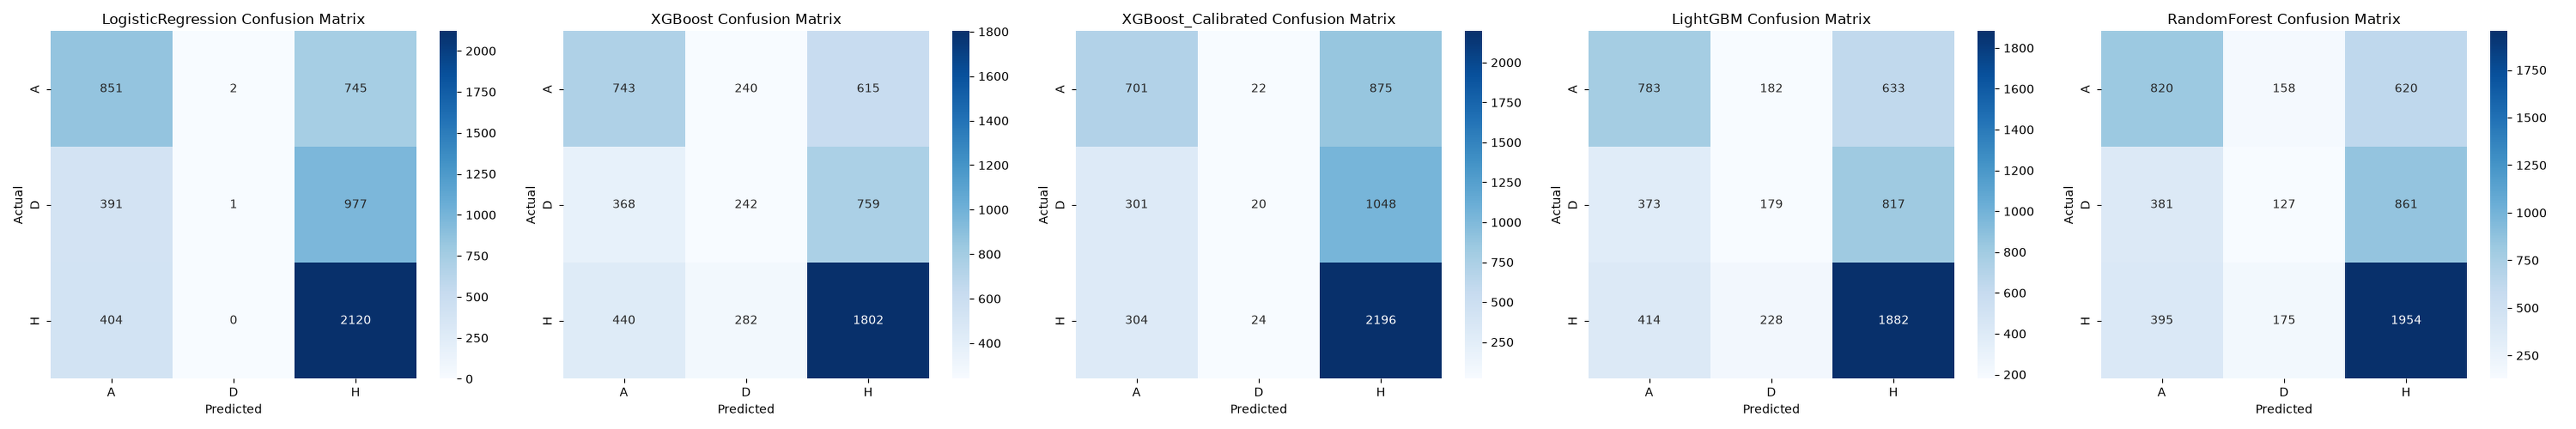
\includegraphics[width=\textwidth]{Fig1.png}
        \caption{Confusion Matrices}
        \label{fig:conf_matrix}
    \end{subfigure}
    \hfill
    \begin{subfigure}[b]{0.48\textwidth}
        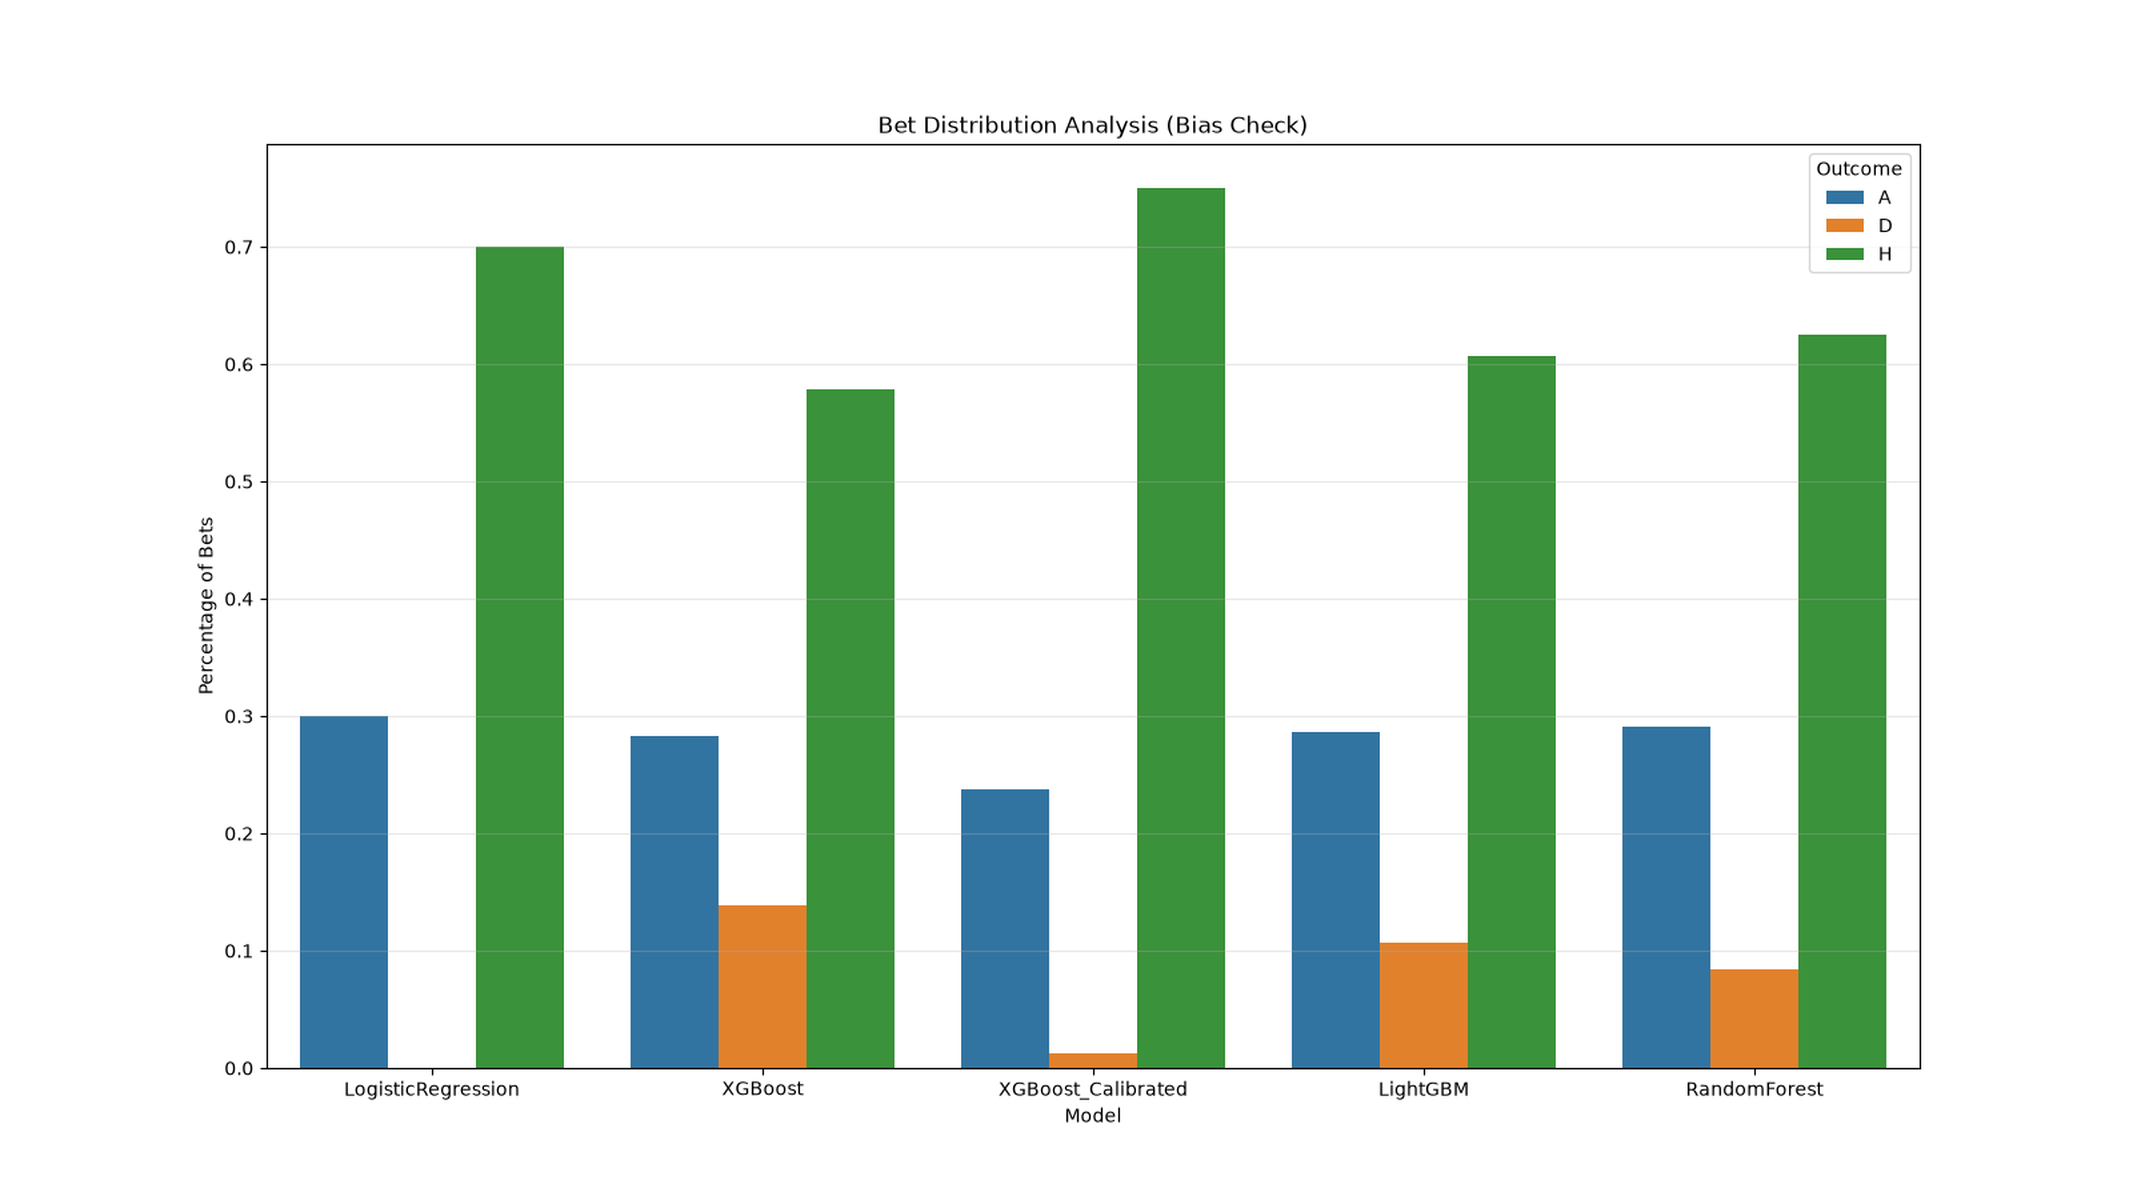
\includegraphics[width=\textwidth]{Fig2.png}
        \caption{Bet Distribution by Outcome}
        \label{fig:bet_dist}
    \end{subfigure}
    \caption{(a) The Confusion Matrices reveal a systemic failure to predict Draws (center column). (b) The Bet Distribution shows the models compensating for this uncertainty by over-betting on the Home Team (right bars), effectively "chasing" the home-field advantage.}
    \label{fig:bias_check}
\end{figure}

The Confusion Matrices (Fig. \ref{fig:conf_matrix}) reveal a flaw: the models are "risk-averse." They almost never successfully predict a Draw, which is typically the outcome with the highest variance but also significant value. Instead, as seen in Fig. \ref{fig:bet_dist}, they aggressively bet on the Home Team. By avoiding the risky Draw calls, the models artificially inflate their accuracy (since Home wins are common) but miss the high-odds opportunities necessary to overcome the bookmaker's margin.

\subsection{The Timeline of Profitability (Alpha Decay)}
While the models were statistically distinct from the market, they were not consistently profitable over the entire 15-year period. When we broke down the returns year by year, a distinct pattern of "Alpha Decay" emerged (Fig. \ref{fig:alpha_decay_combined}).

\begin{itemize}
    \item \textbf{Phase I: Market Inefficiency (2006–2014):} In the earlier years of our simulation, the XGBoost model showed strong performance. It generated positive returns in several seasons, peaking with an +18.31\% return on investment in 2014. During this era, the "edge" was real. Crucially, the model's advantage during this period was large enough to overcome the "vigorish" (the bookmaker's built-in fee), resulting in net profit.
    \item \textbf{Phase II: The Leicester Anomaly and Market Correction (2015–2021):} The profitability trend violently reversed starting in the 2015-2016 season. This corresponds to what is widely considered the most unpredictable season in Premier League history, where 5,000-to-1 underdogs Leicester City won the title alongside a historic, collective underperformance by the traditional "Big 6" clubs. A historical machine learning model trained on 2000–2014 data heavily assumes that established giants consistently defeat smaller clubs. The 2015-16 season shattered these learned heuristics, causing severe financial drawdowns as the models confidently and repeatedly bet on failing favorites. Following this anomaly, returns became highly volatile and failed to sustain growth, suffering another significant concept-drift drawdown during the empty-stadium matches of 2020 (-13.24\%).
\end{itemize}

Given this violent reversal in 2015, a central question is whether the Leicester City anomaly represented a permanent structural break in football forecasting, or merely a massive outlier masking a gradual tightening of market efficiency. To test this formally, we ran an OLS-based CUSUM test for structural breaks on the year-over-year ROI. The test returned a p-value of 0.9940, failing to reject the null hypothesis of structural stability. 

This confirms that there was no singular, permanent mathematical "shock" to the market. Instead, the timeline aligns perfectly with Lo's (2004) Adaptive Markets Hypothesis. Following Leicester's victory, the 2016-17 season saw the implementation of a historic \pounds 5.1 billion domestic television rights deal. As noted in sports economics literature \cite{peeters2011}, this massive influx of evenly distributed broadcast revenue significantly leveled the financial playing field for mid-table clubs, fundamentally altering the league's competitive balance. As bookmakers integrated their own advanced algorithms to account for this new parity, the localized inefficiencies that our models exploited in Phase I were gradually squeezed out of the market.

To verify that the models themselves didn't simply degrade in quality, we analyzed the stability of their error rates. We found that the Mean Brier Error remained remarkably stable (0.242 in the early era vs. 0.234 in the late era). Crucially, a Kolmogorov-Smirnov (KS) test on the error distributions yielded a p-value of 0.29. This confirms that the model's predictive distribution did not fundamentally change; rather, the market's efficiency threshold simply increased.

\begin{figure}[htbp]
    \centering
    \begin{subfigure}[b]{0.48\textwidth}
        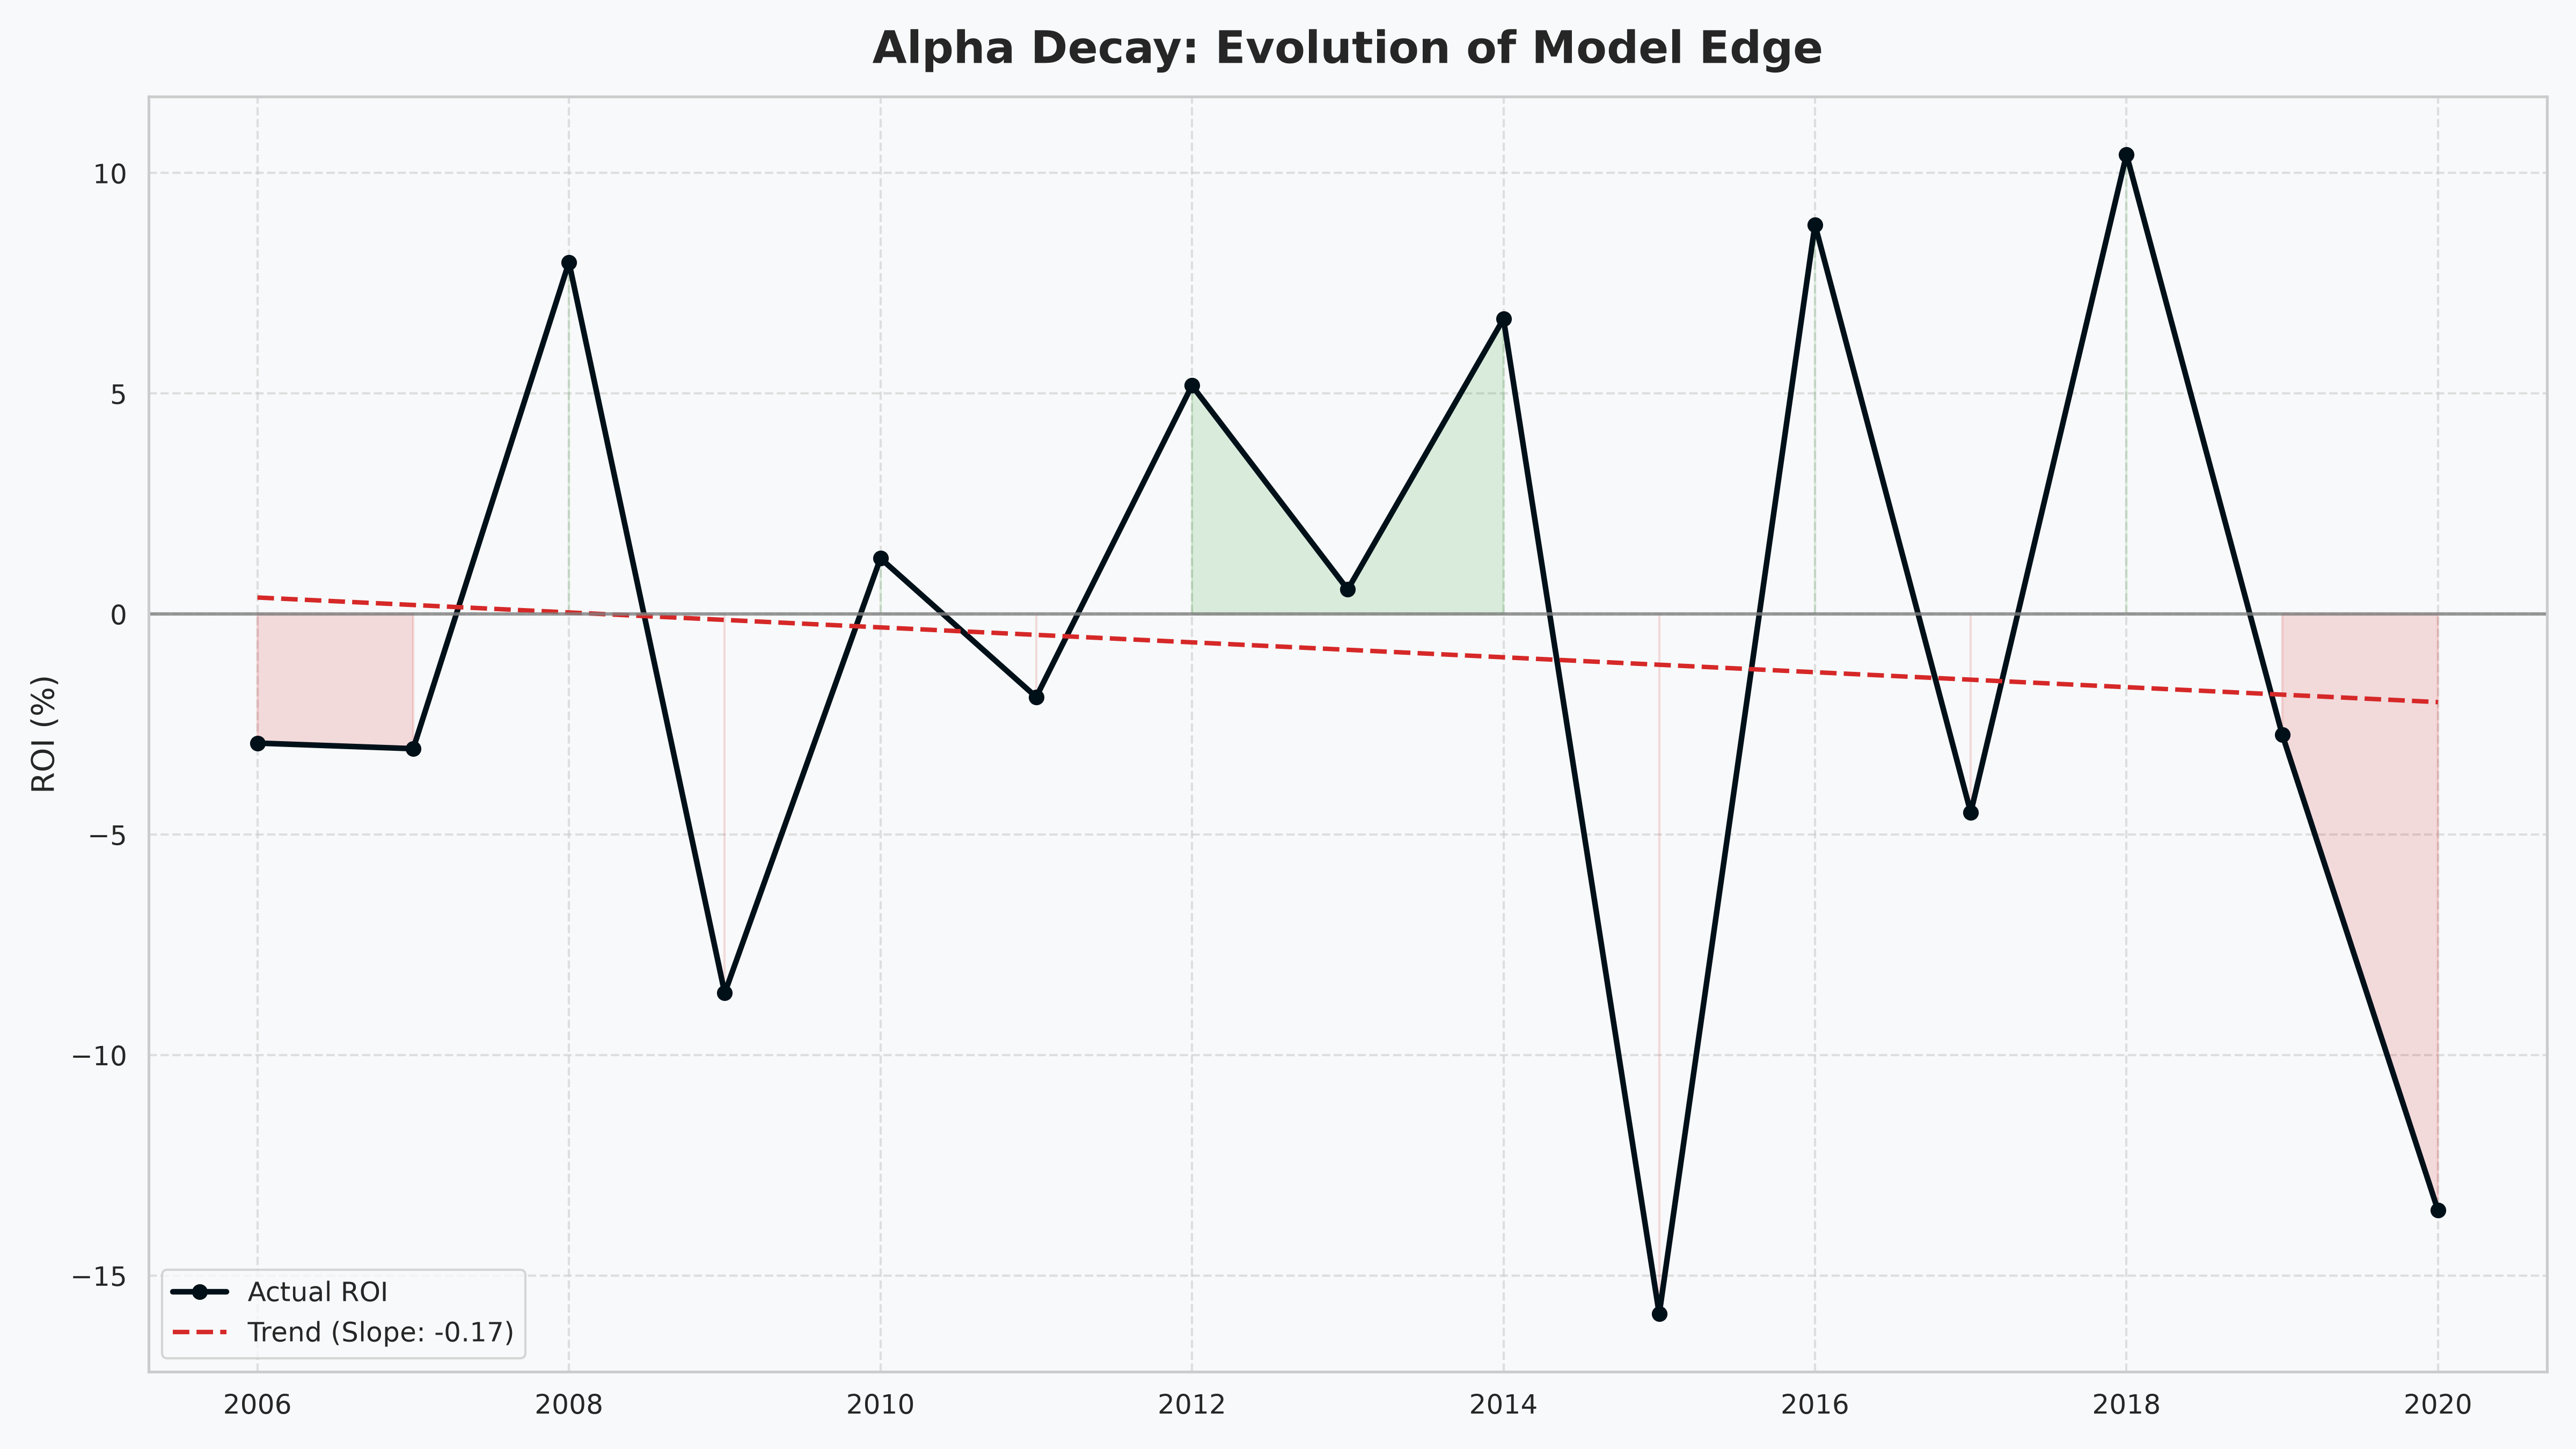
\includegraphics[width=\textwidth]{Fig3.png}
        \caption{Long-term Trend}
        \label{fig:alpha_decay_trend}
    \end{subfigure}
    \hfill
    \begin{subfigure}[b]{0.48\textwidth}
        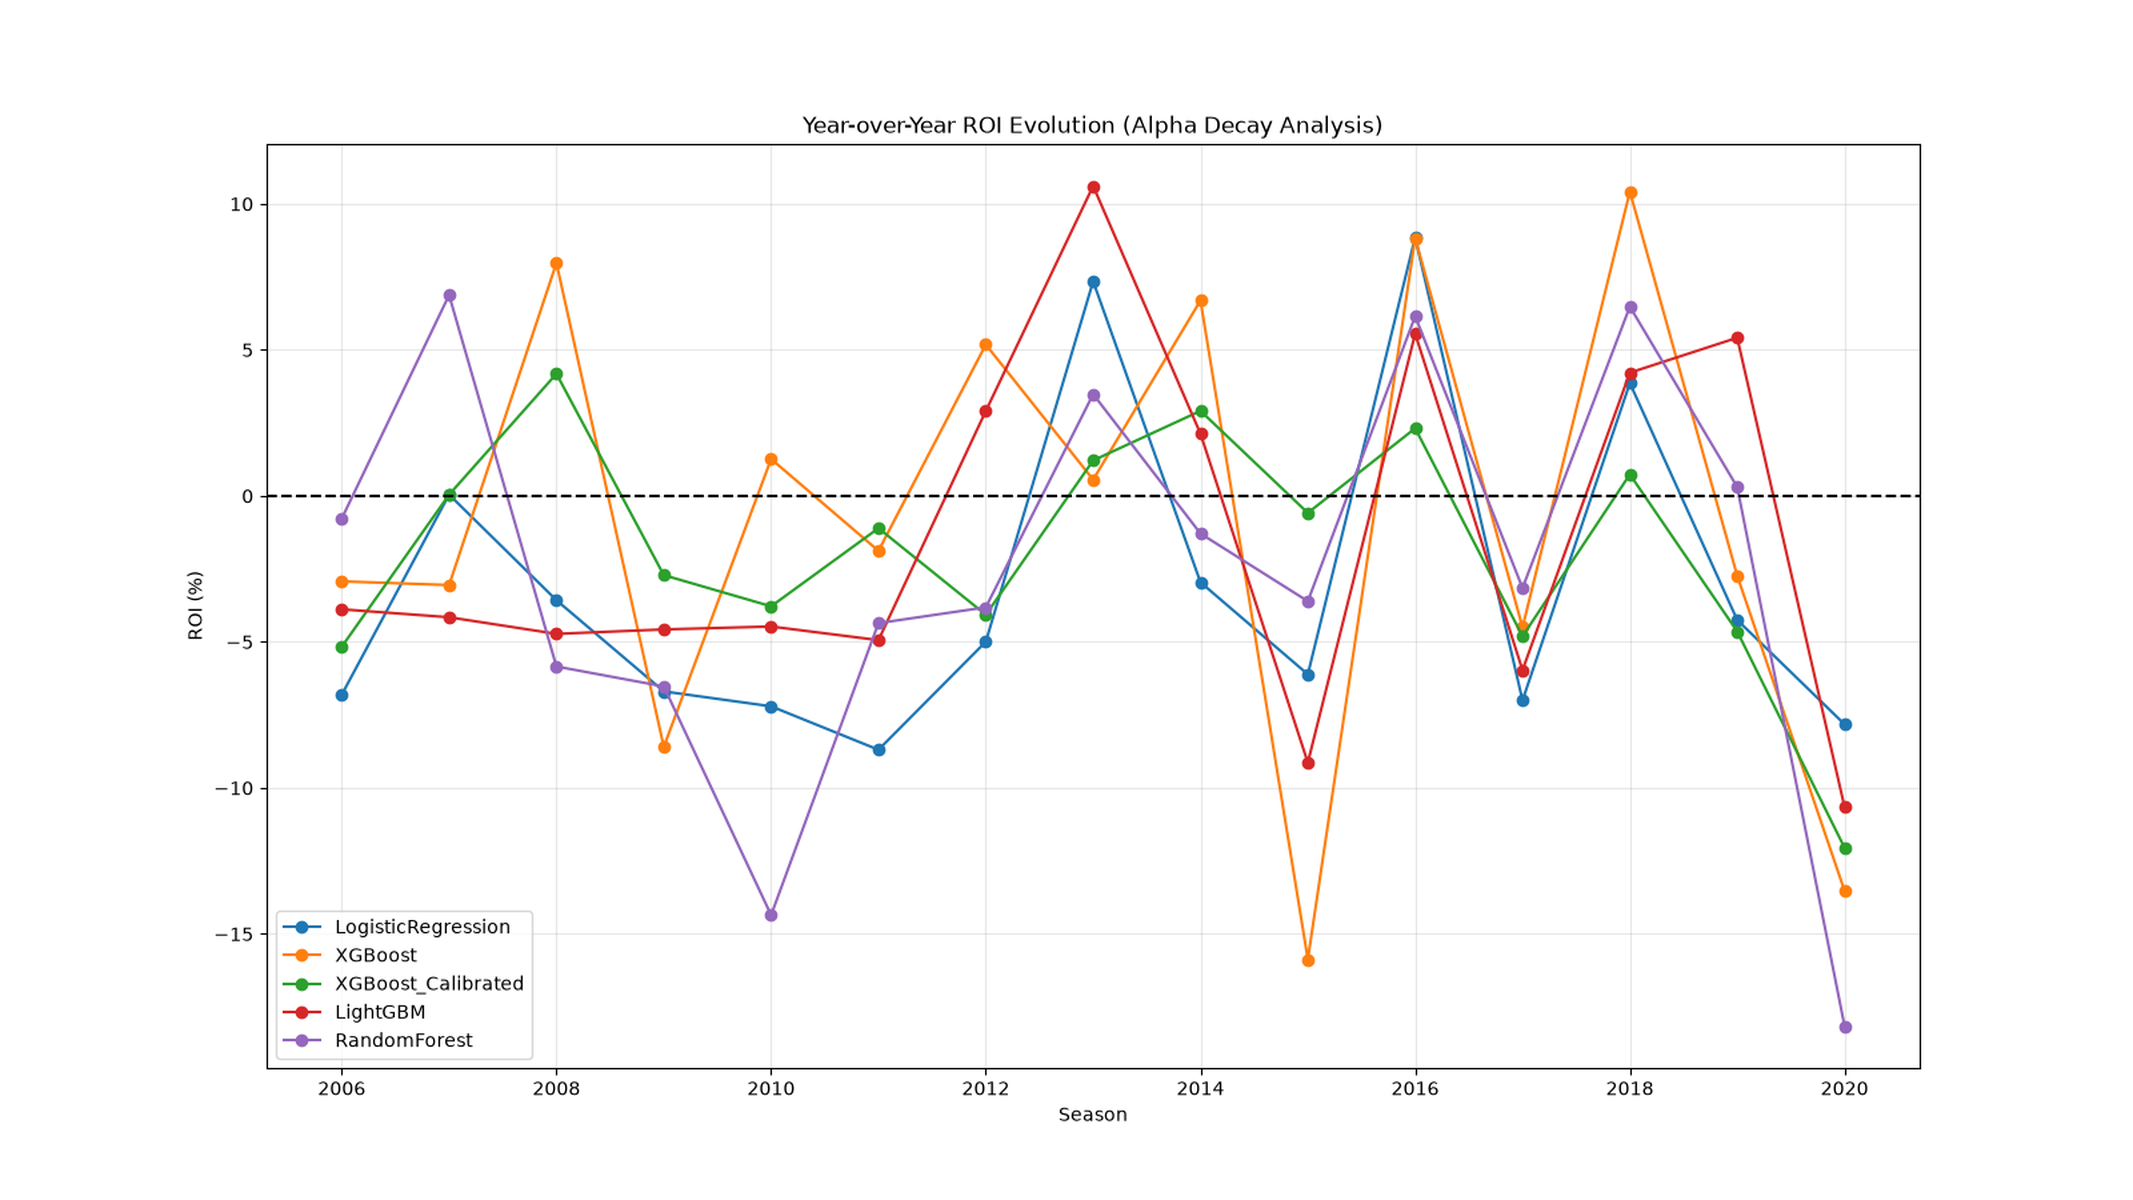
\includegraphics[width=\textwidth]{Fig4.png}
        \caption{Year-over-Year Volatility}
        \label{fig:alpha_decay_lines}
    \end{subfigure}
    \caption{Alpha Decay Analysis. (a) The stylized trend showing the "Golden Age" (green) vs the "Efficient Era" (red). (b) The raw performance lines for all three models, showing the specific volatility and the sharp drop-off for XGBoost (blue) after 2014.}
    \label{fig:alpha_decay_combined}
\end{figure}

We can see this impact most clearly when looking at the cumulative wealth over time (Fig. \ref{fig:wealth}). If you had started using the XGBoost model in 2006, you would have seen a steady climb in profits. However, the data reveals a persistent "Alpha Decay." A linear trend analysis shows the model's edge over the bookmaker degrading consistently as the market became more efficient.

\begin{figure}[H]
    \centering
    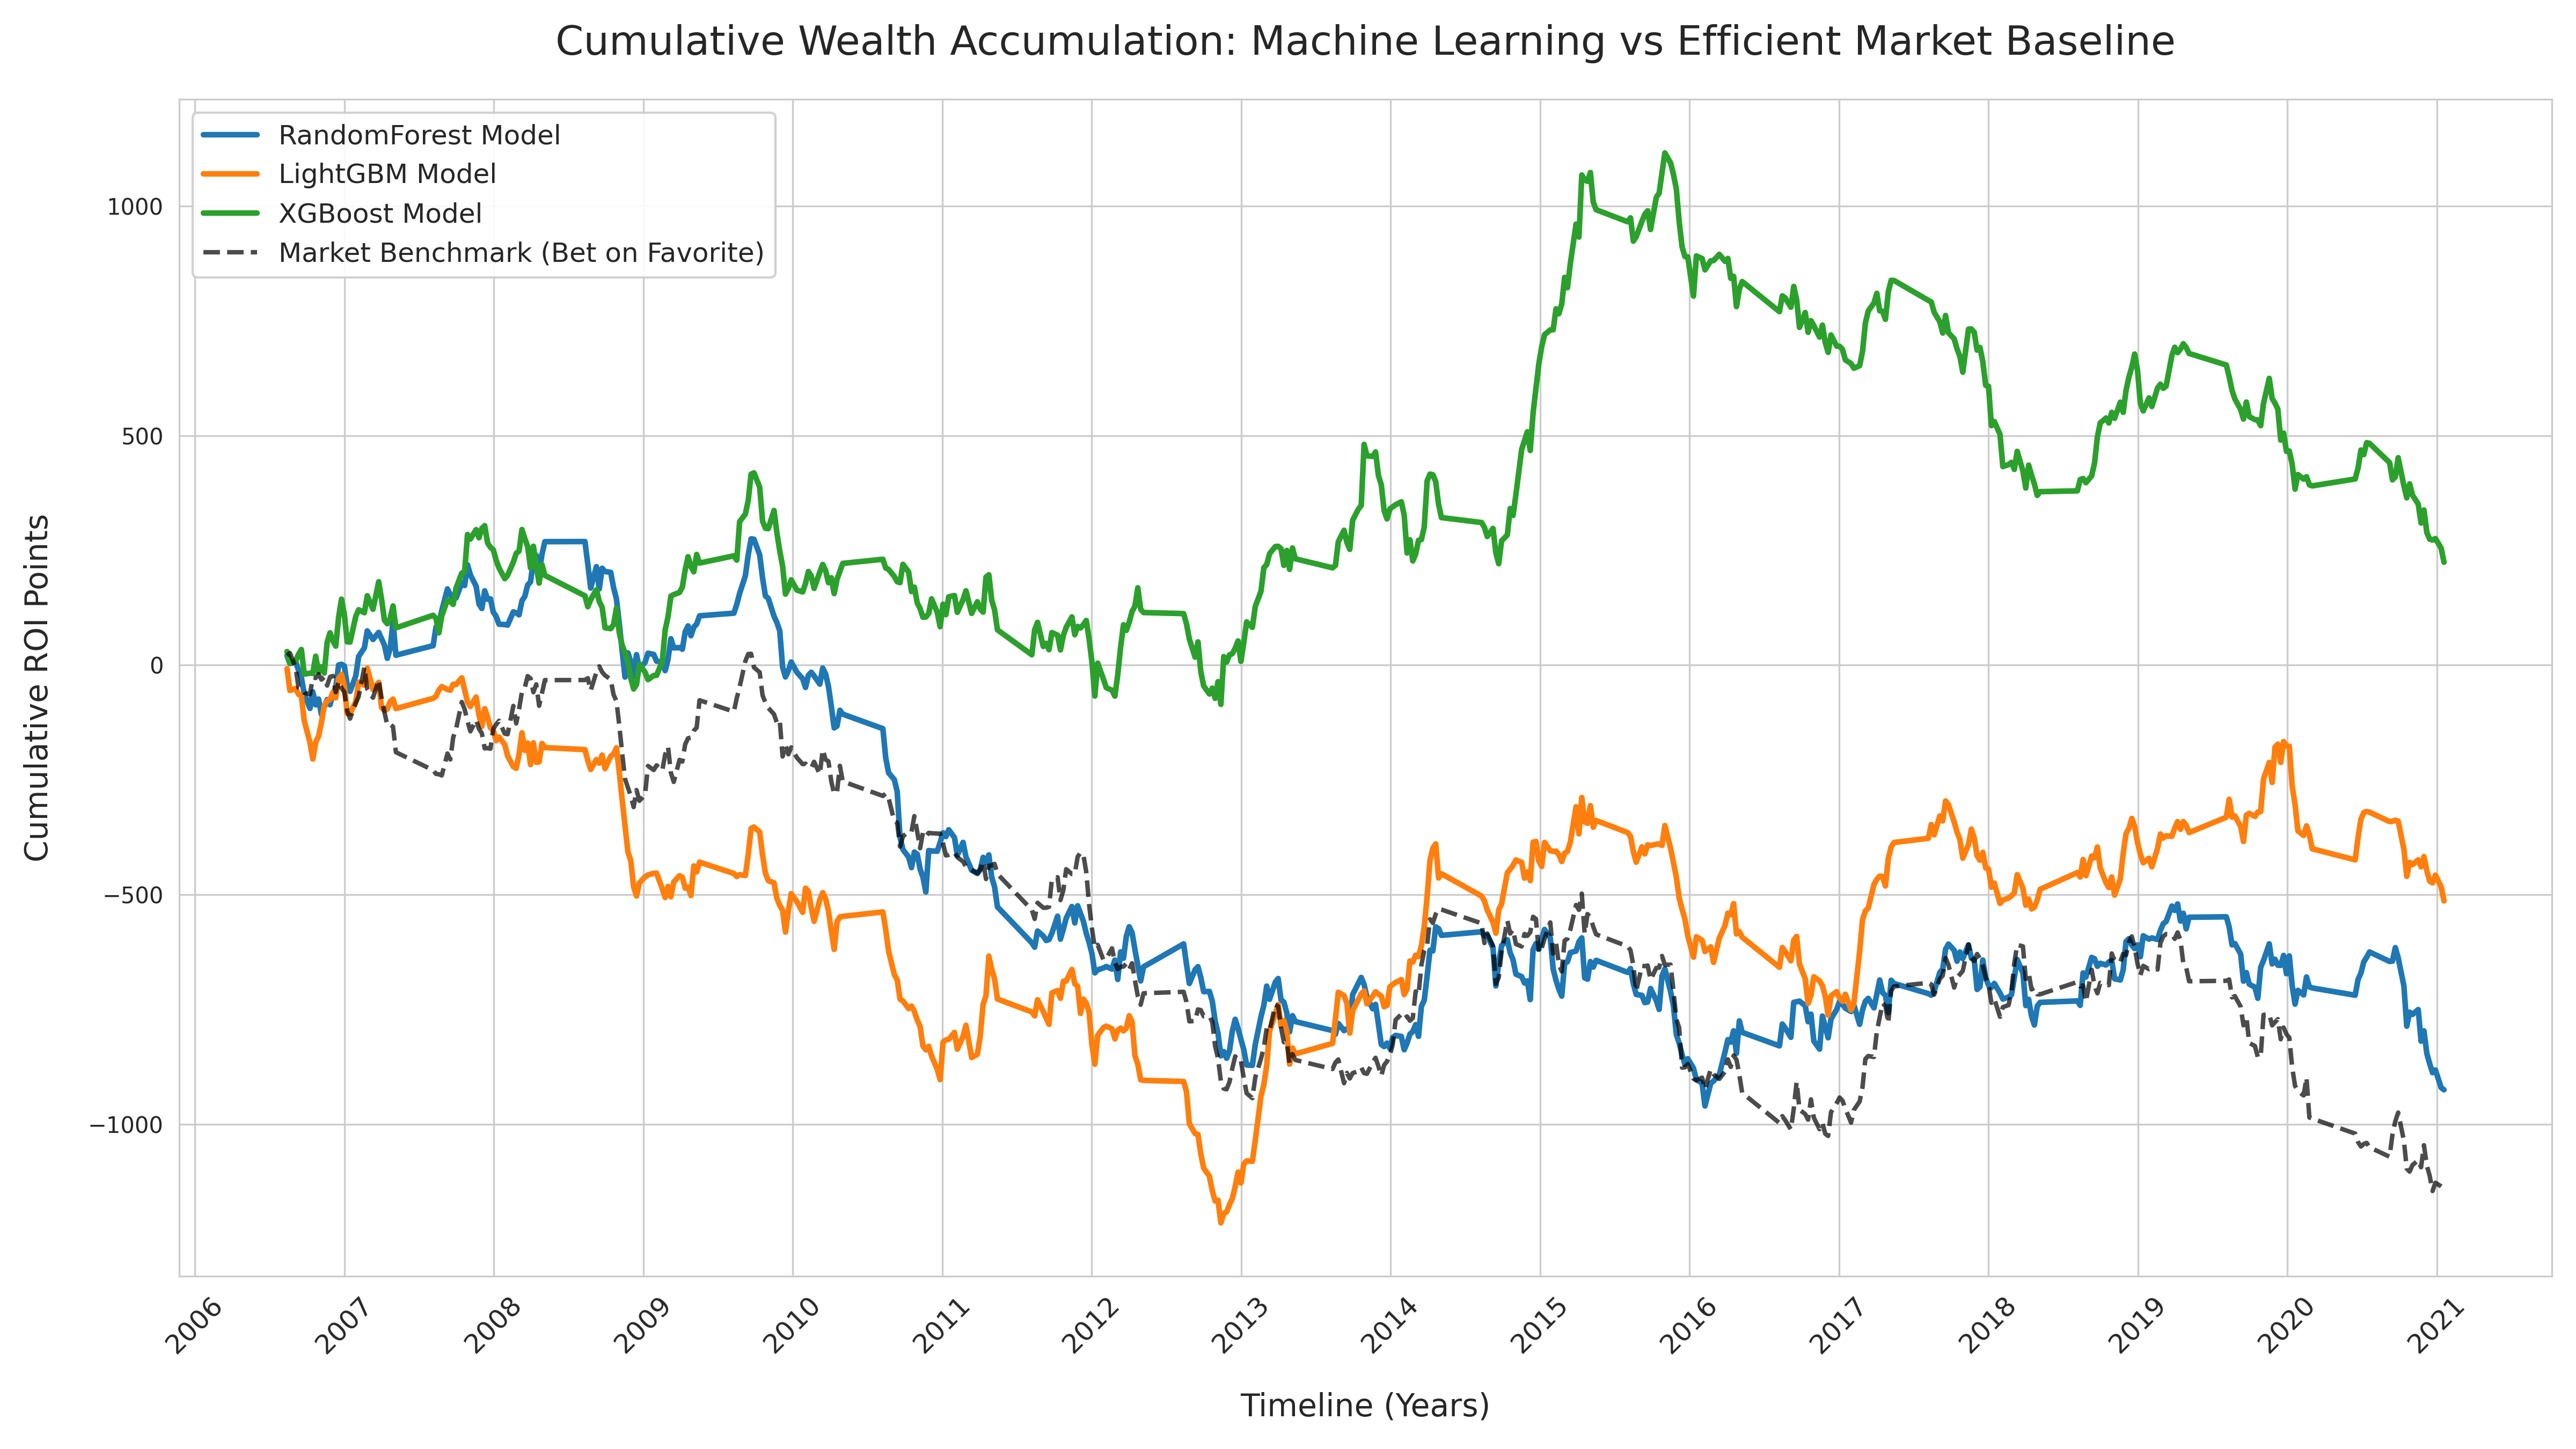
\includegraphics[width=1.0\textwidth]{Fig5.png}
    \caption{Cumulative Wealth Accumulation. The green line (XGBoost) illustrates the "Golden Age" of sports betting, showing strong growth until 2015. After that point, the line flattens and becomes volatile, struggling to beat the simple "Market Benchmark" (grey dashed line) of just betting on the favorite.}
    \label{fig:wealth}
\end{figure}

\subsection{The Cure for Overconfidence: Calibration and Fractional Staking}
The most critical finding of our study lies in resolving the difference between being "accurate" and being "calibrated." We simulated the Kelly Criterion \cite{kelly1956}, a famous mathematical formula that optimally sizes bets based on the model's computed edge. 

As discussed in Section 2, the Kelly formula is highly sensitive to parameter uncertainty. When we applied it to the uncalibrated XGBoost model (which suffered a severe Expected Calibration Error of 0.145), the results were catastrophic. Because the model chronically overestimated its own edge, the standard "Full Kelly" strategy immediately went bankrupt (\$0.00). Even when applying a highly conservative "Fractional Kelly" (staking only 10\% of the recommended amount to provide a margin of safety), the uncalibrated model still destroyed 73\% of its starting capital, plummeting from \$10,000 to \$2,705.

However, when we applied post-hoc Isotonic Regression to mathematically correct the model's overconfidence, the financial trajectory completely inverted. The calibration process successfully dropped the ECE from 0.145 to a highly robust 0.028, aligning the model's internal confidence with external reality \cite{zadrozny2002}. While the Calibrated model still went bankrupt under the aggressive Full Kelly strategy—confirming MacLean et al.'s (2010) warning that Full Kelly cannot survive the inherent variance of sports \cite{maclean2010}—the combination of Isotonic Calibration and a 10\% Fractional Kelly strategy successfully preserved capital. It yielded a final bankroll of \$10,599 (a +6\% net profit over the baseline).

This finding explicitly resolves a central tension in sports forecasting literature. Neither machine learning accuracy nor risk-management formulas are sufficient on their own to overcome the bookmaker's margin (the vigorish). In a highly efficient, adversarial market, long-term survival is only possible through a dual approach: applying strict probability calibration to mathematically prevent theoretical over-betting, combined with fractional staking to physically absorb real-world parameter uncertainty.

\begin{figure}[H]
    \centering
    \begin{subfigure}[b]{0.48\textwidth}
        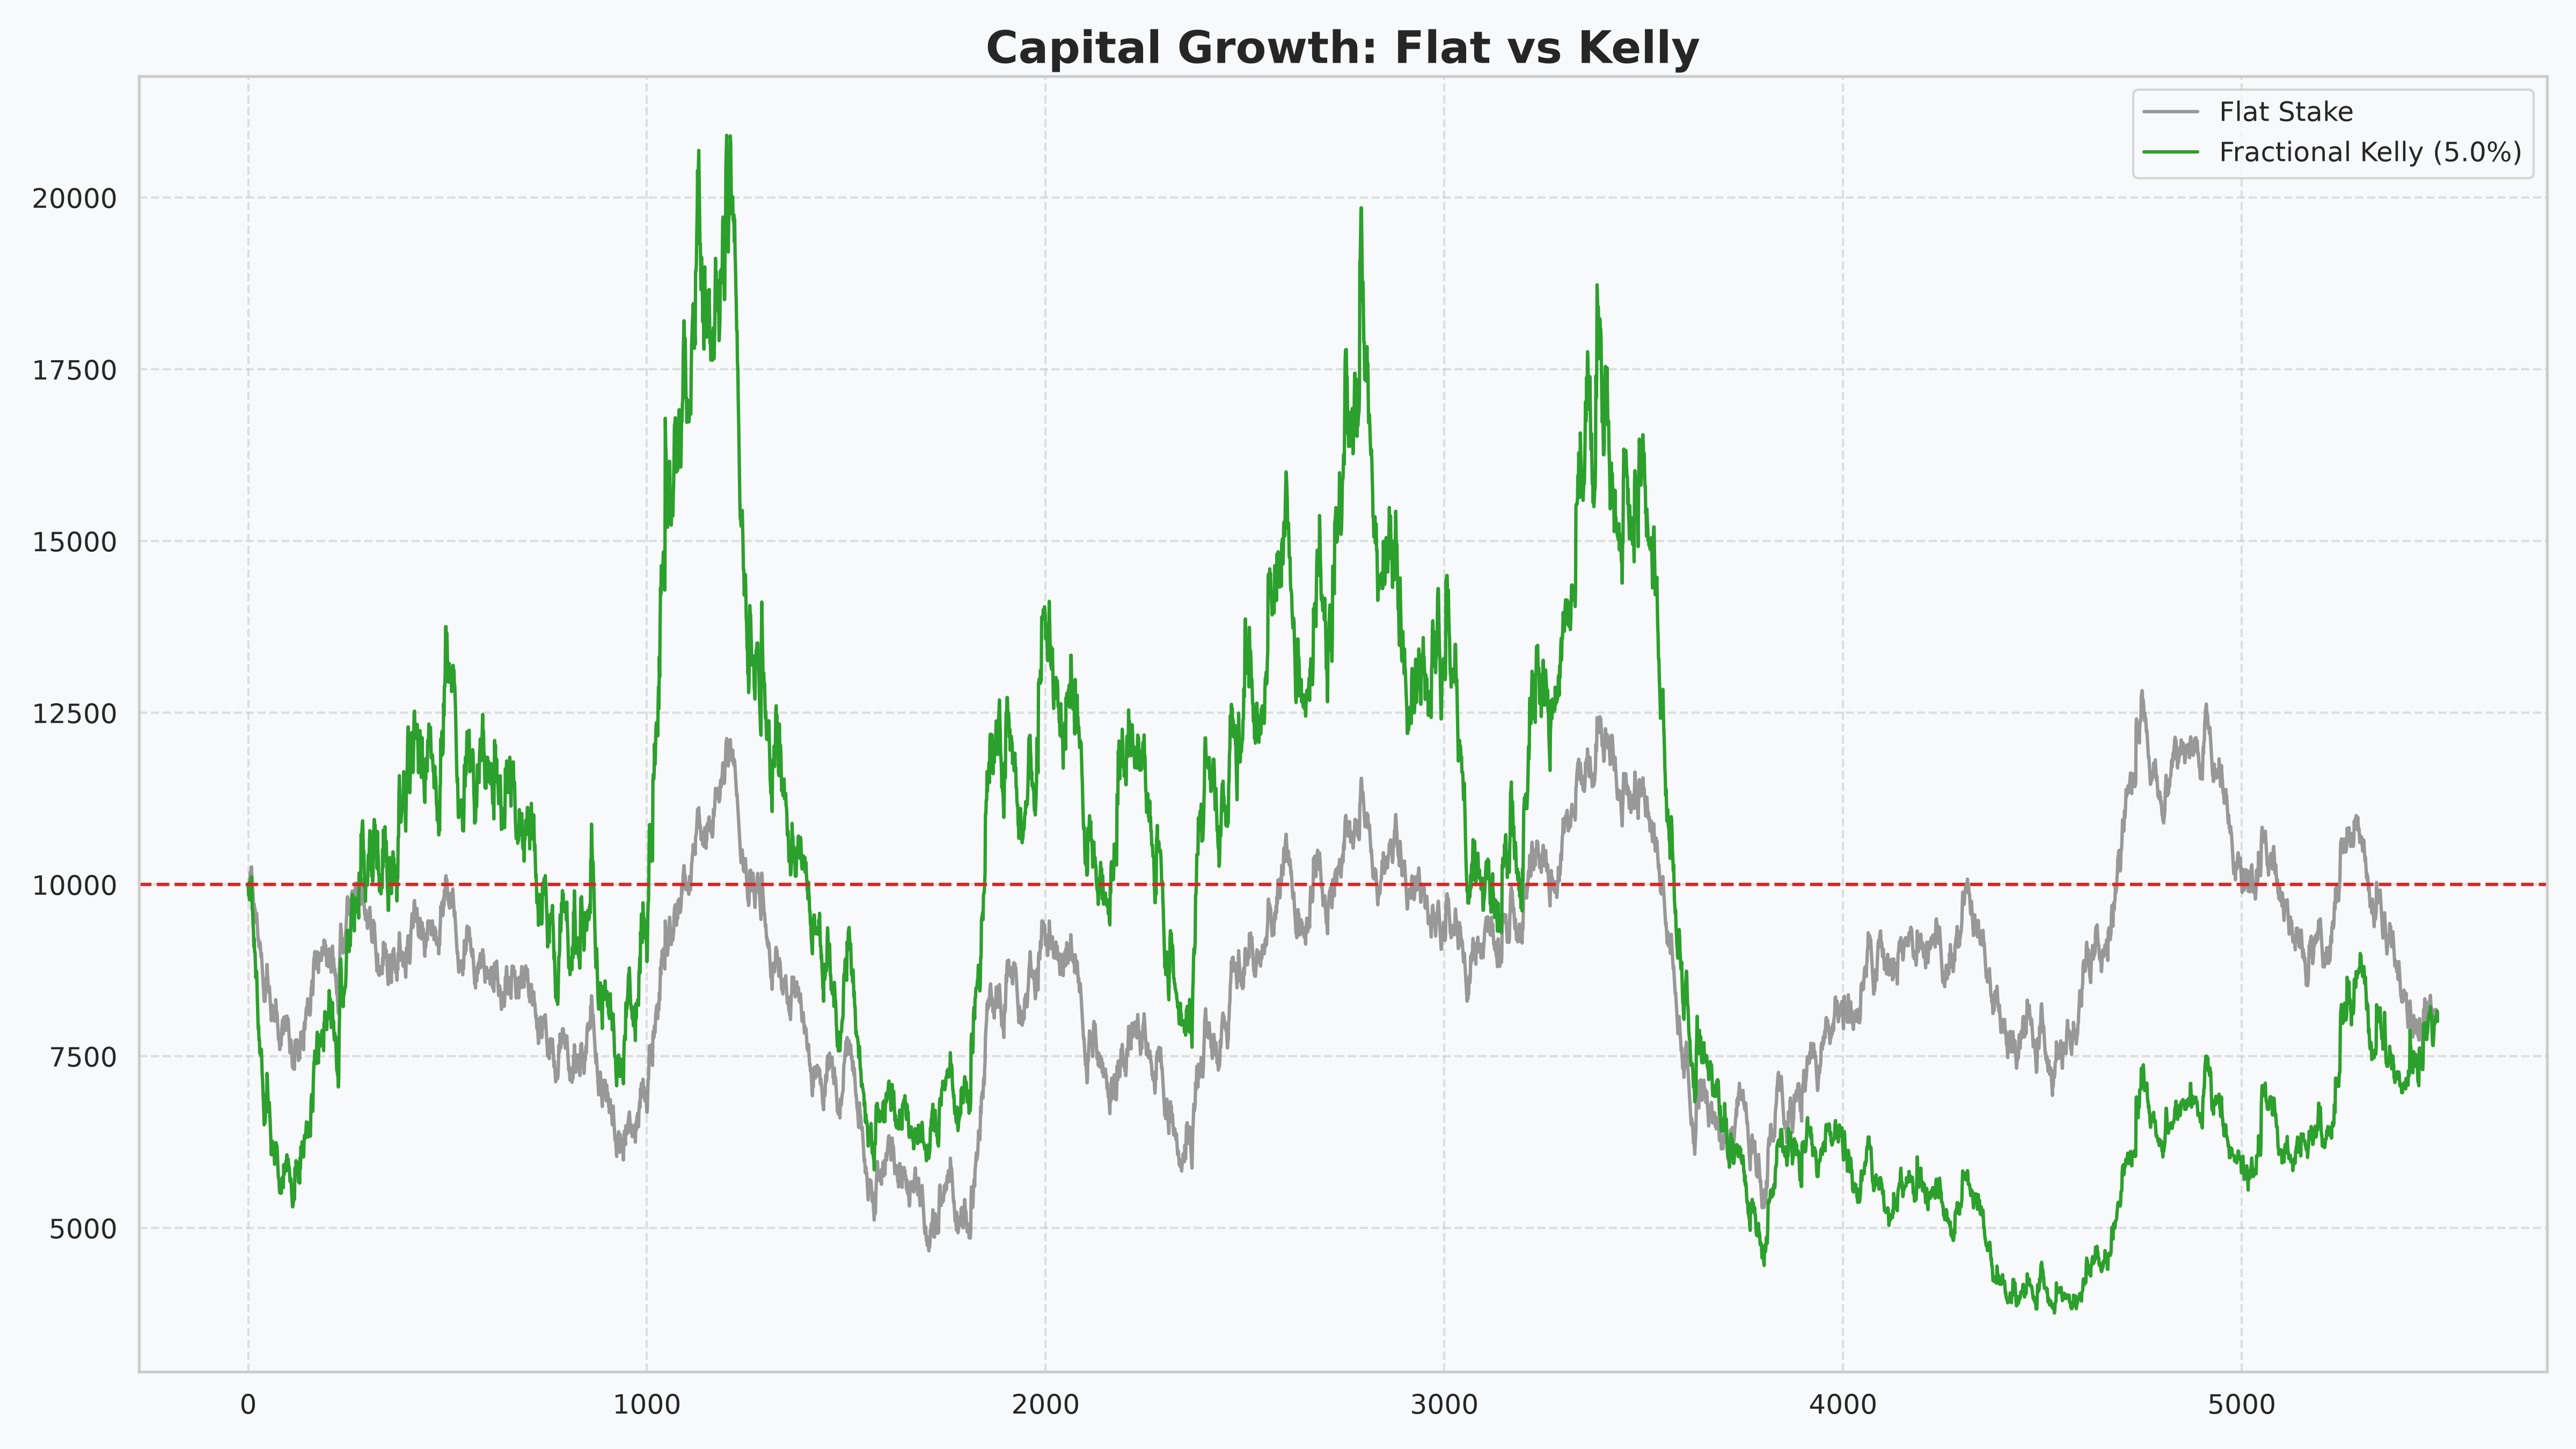
\includegraphics[width=\textwidth]{Fig6.png}
        \caption{Capital Growth: Flat vs. Fractional Kelly}
        \label{fig:kelly_flat}
    \end{subfigure}
    \hfill
    \begin{subfigure}[b]{0.48\textwidth}
        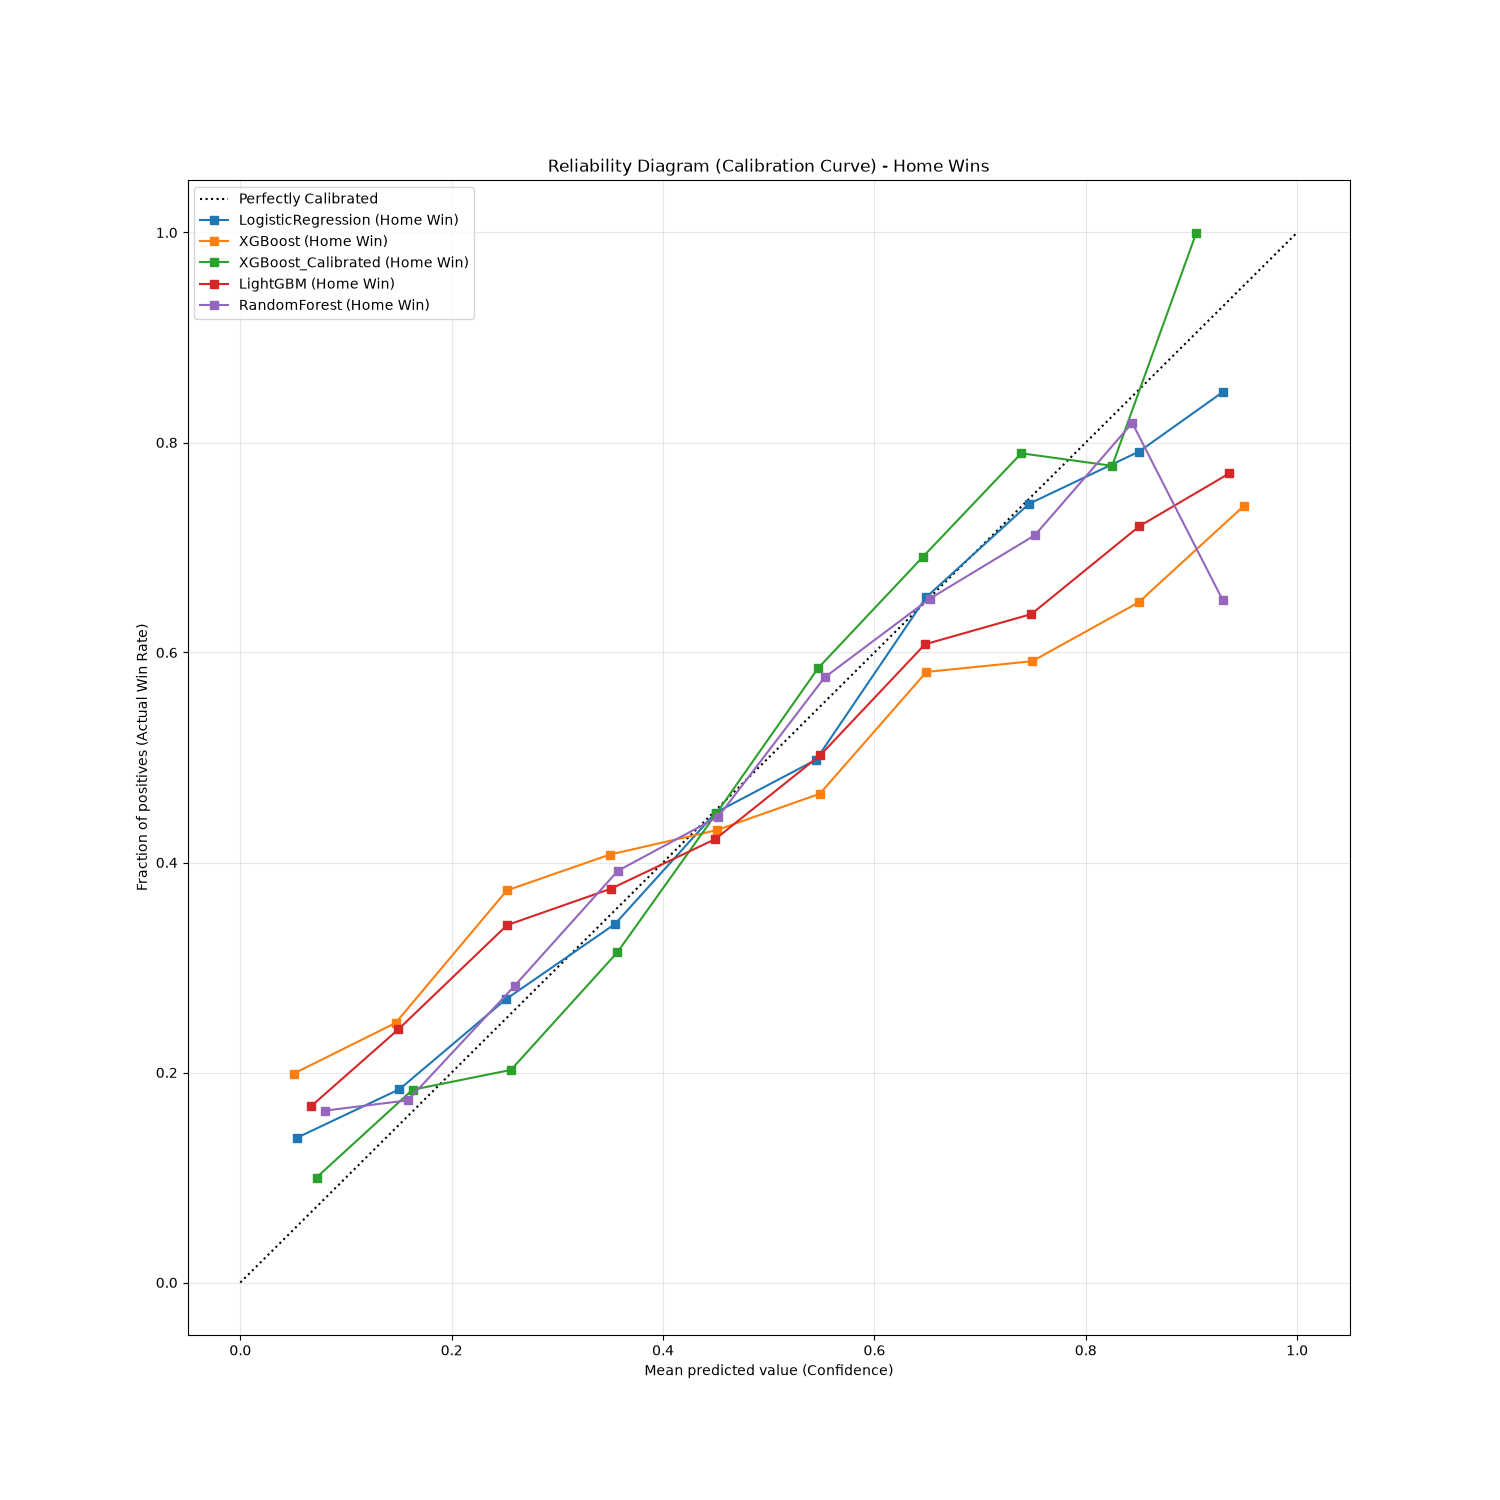
\includegraphics[width=\textwidth]{Fig7.png}
        \caption{Calibration Curve}
        \label{fig:calibration}
    \end{subfigure}
    \caption{(a) Without calibration, Fractional Kelly strategies rapidly deteriorate due to parameter uncertainty. (b) The calibration curve confirms this: the base model's confidence lines are mostly below the "Perfectly Calibrated" dotted line, meaning it was consistently too optimistic before Isotonic Regression was applied.}
\end{figure}

\subsection{Ablation Study and Feature Importance}
To understand what the AI was actually looking at to make its predictions, we analyzed the SHAP Feature Importance (Fig. \ref{fig:shap}). The results showed that the Home Odds and Away Odds were the overwhelming primary drivers, vastly outweighing fundamental team performance metrics like 'Away Avg Shots' or 'Home Points'.

To rigorously test this hypothesis, we conducted an Ablation Study comparing an "Odds-Only" model (trained strictly on the 3 market prices) against a "Fundamentals-Only" model (trained strictly on the 10 rolling-window team metrics). The Fundamentals-Only model suffered a catastrophic collapse in both accuracy and log-loss compared to the Odds-Only variant. This explicitly confirms that the vast majority of the models' predictive power comes from reading the bookmaker's mind (the odds) rather than reading the game itself (the fundamentals). The bookmaker's price already efficiently encodes the fundamental metrics.

\begin{figure}[H]
    \centering
    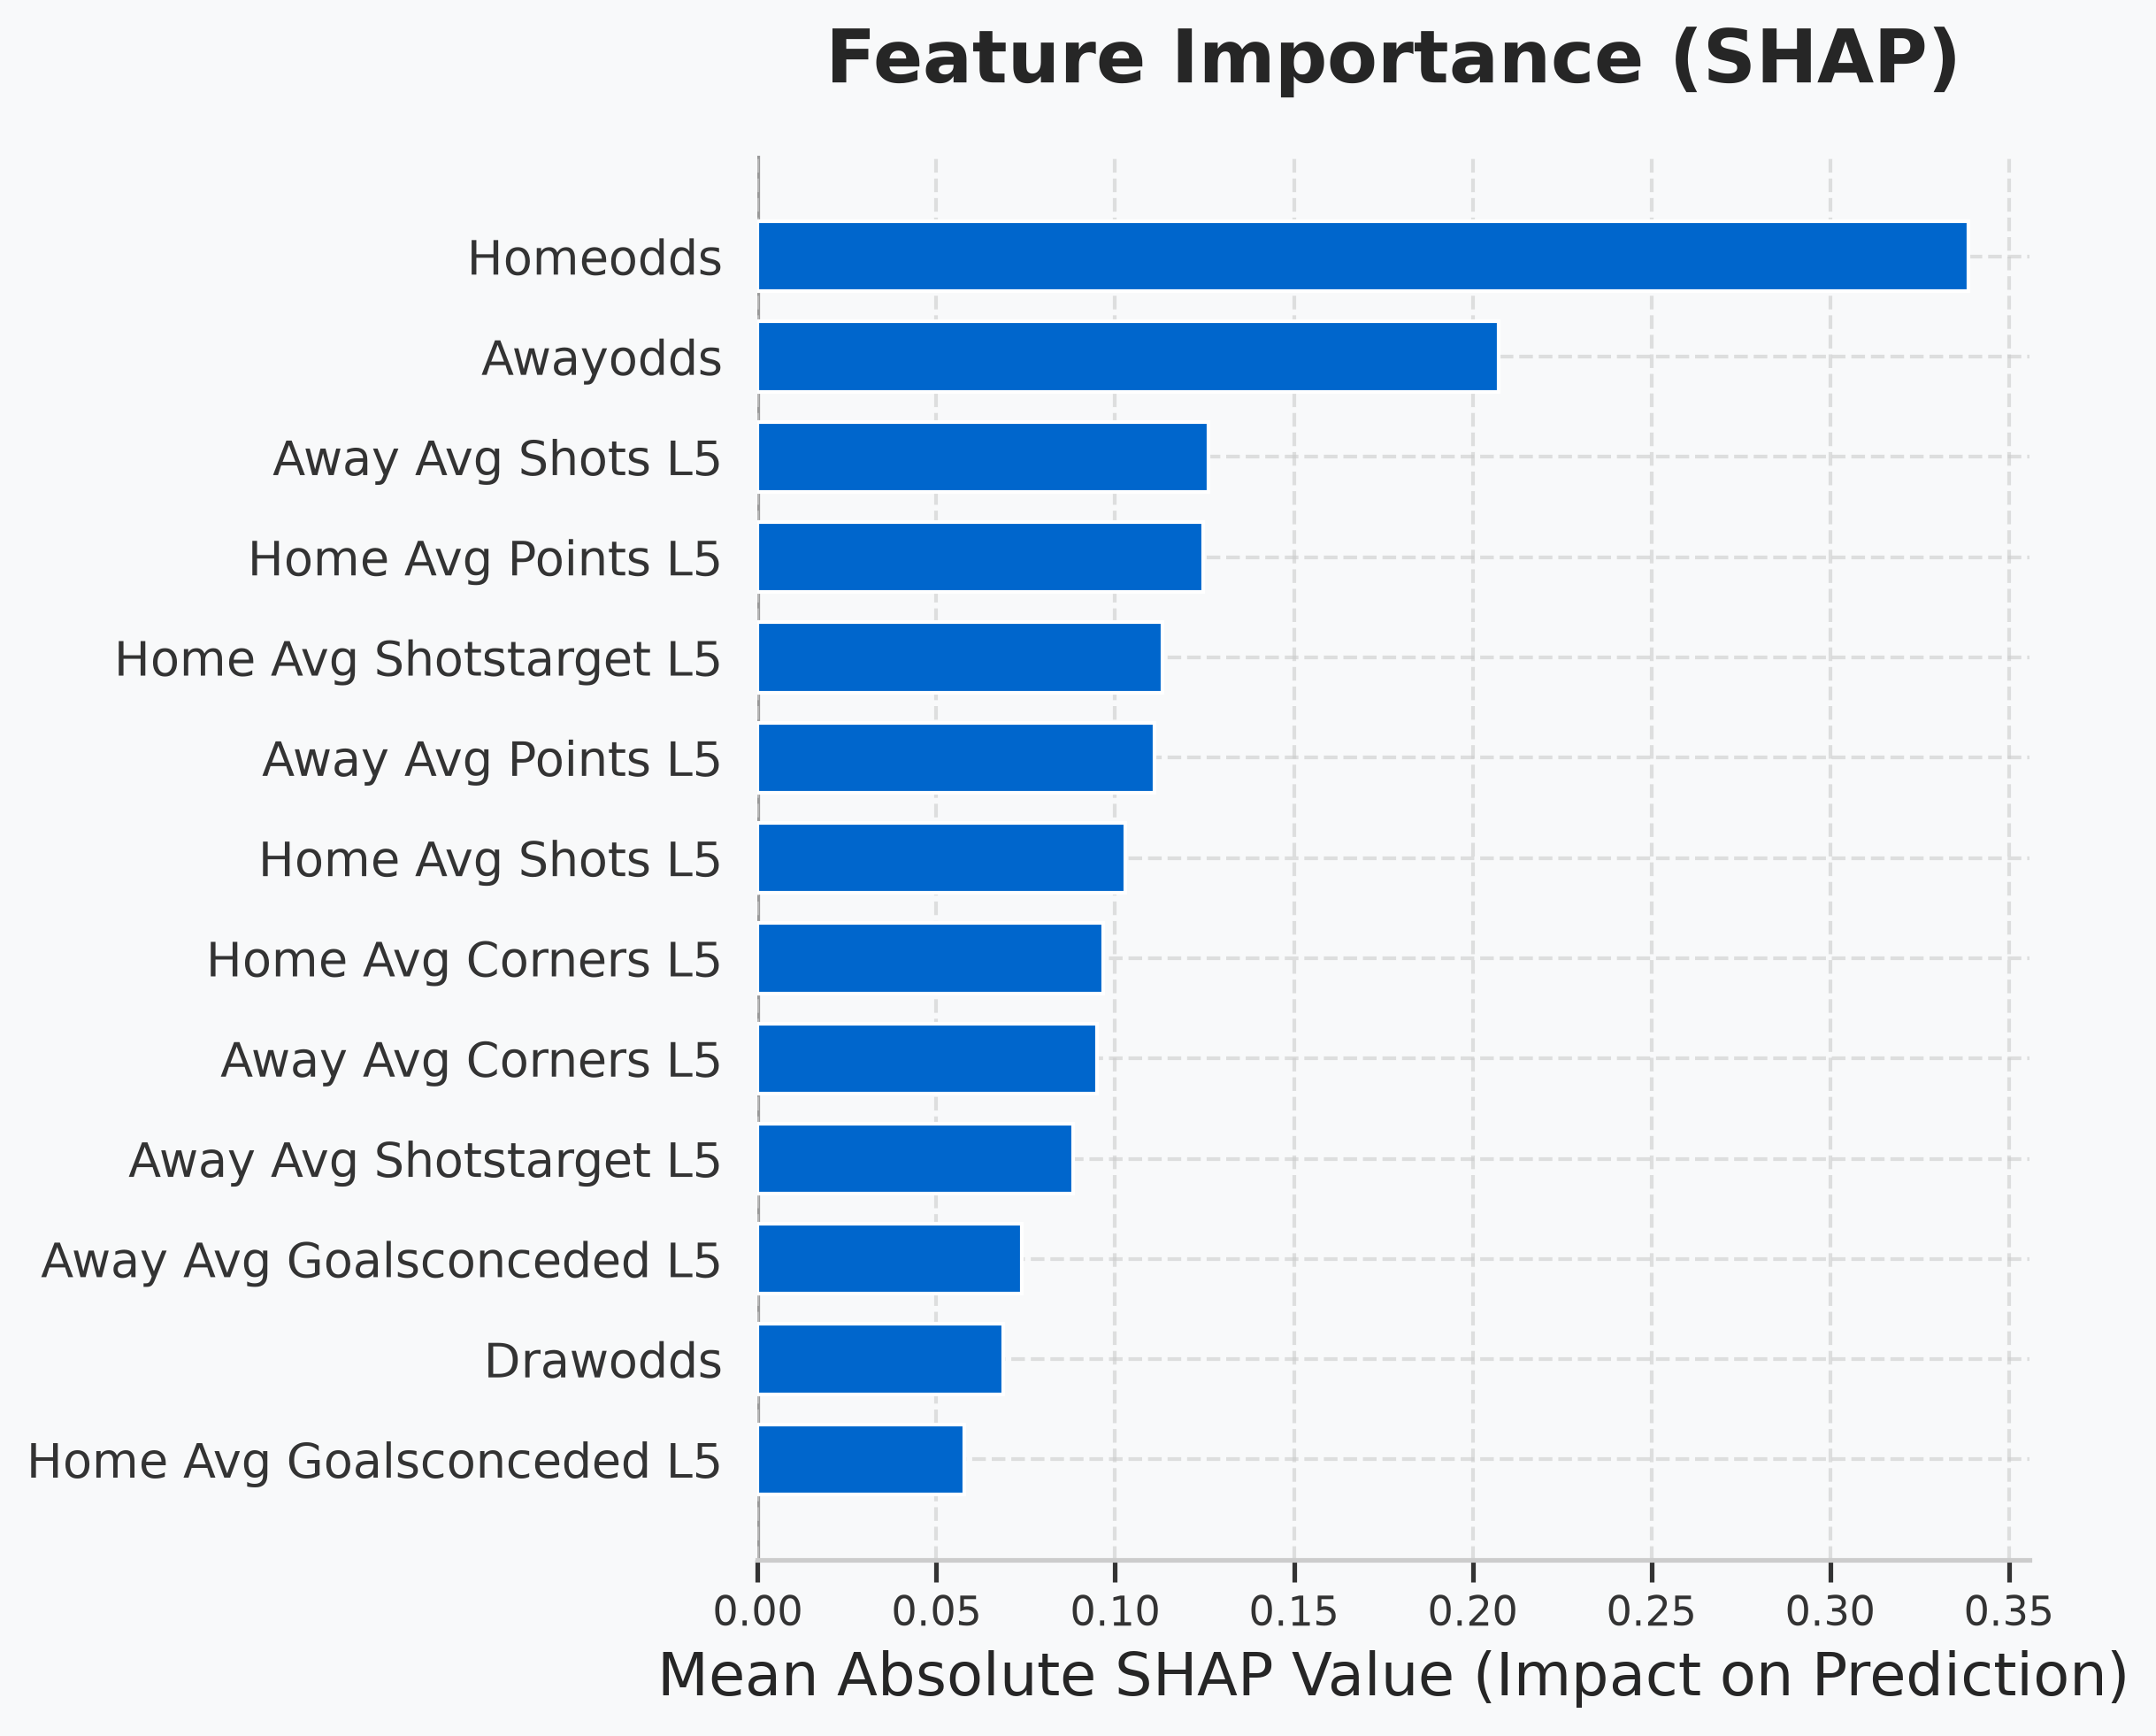
\includegraphics[width=0.8\textwidth]{Fig8.png}
    \caption{SHAP Feature Importance. The blue bars represent how much each data point contributed to the AI's decision. The most important feature was "HomeOdds"—the price set by the bookmaker. This proves the AI relies on market consensus rather than independent sports analysis.}
    \label{fig:shap}
\end{figure}

\subsection{Risk Assessment via Monte Carlo Simulation}
Averages can be misleading. Just because the "average" simulation made a small profit doesn't mean a real person would. To see the true risk, we ran 20,000 simulations of the best performing strategy (XGBoost) to see the range of possible outcomes for a bettor.

The results (Fig. \ref{fig:monte_carlo_hist}) were sobering. While the strategy was profitable 58.3\% of the time, the risk profile reveals hidden dangers. The strategy achieved a Sortino Ratio of 0.38, but the risk profile is dangerous. As shown in Figure \ref{fig:monte_carlo_hist}, \textbf{41.7\%} of all simulated lifetimes failed to generate a profit, with \textbf{5.1\%} resulting in total bankruptcy. Furthermore, the 95\% Value at Risk (VaR) analysis shows significant downside potential in the worst-case scenarios.

\begin{figure}[H]
    \centering
    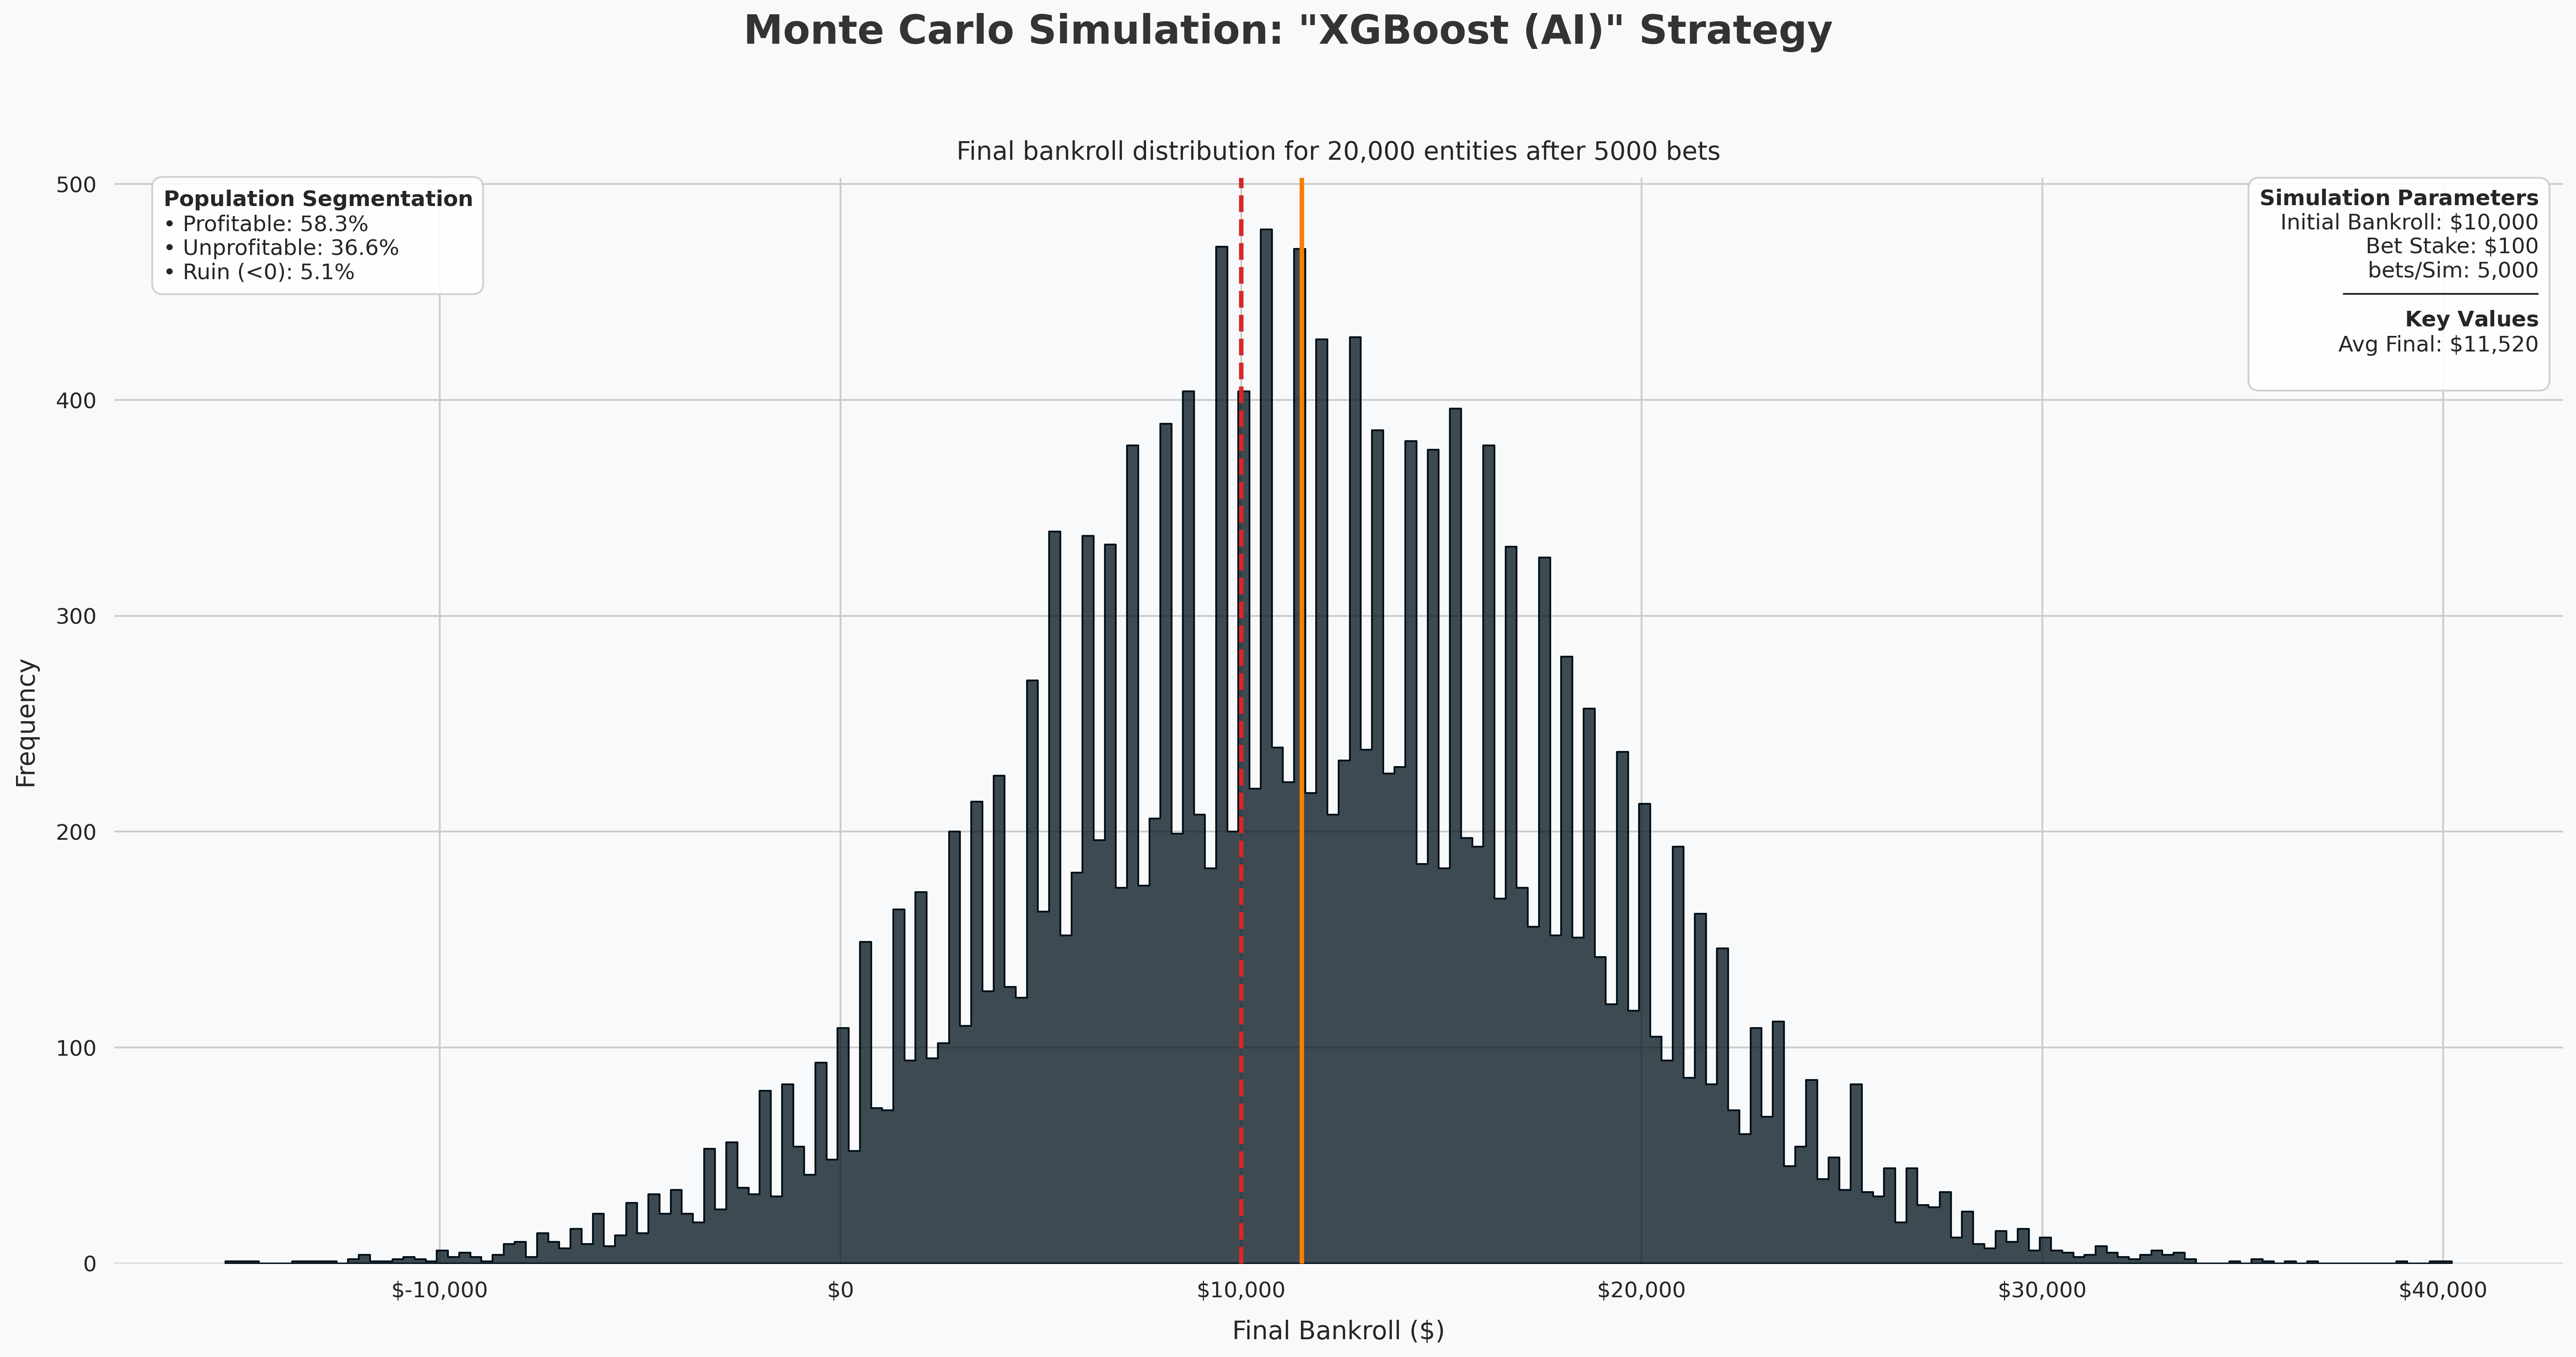
\includegraphics[width=1.0\textwidth]{Fig9.png}
    \caption{Monte Carlo Simulation (XGBoost). This histogram shows the final bankroll for 20,000 simulated players. While the average (orange line) is profitable at \$11,520, the distribution is wide. The red dashed line shows the starting \$10,000. Anyone to the left of that line lost money.}
    \label{fig:monte_carlo_hist}
\end{figure}

When we compare this to standard human strategies (Fig. \ref{fig:comparative_kde}), we see that the AI (green curve) shifts the outcomes slightly to the right compared to simply betting on the Favorite (blue) or the Home Team (red). It doesn't guarantee a win, but it tilts the odds slightly in your favor—just not enough to overcome the variance for everyone.

\begin{figure}[H]
    \centering
    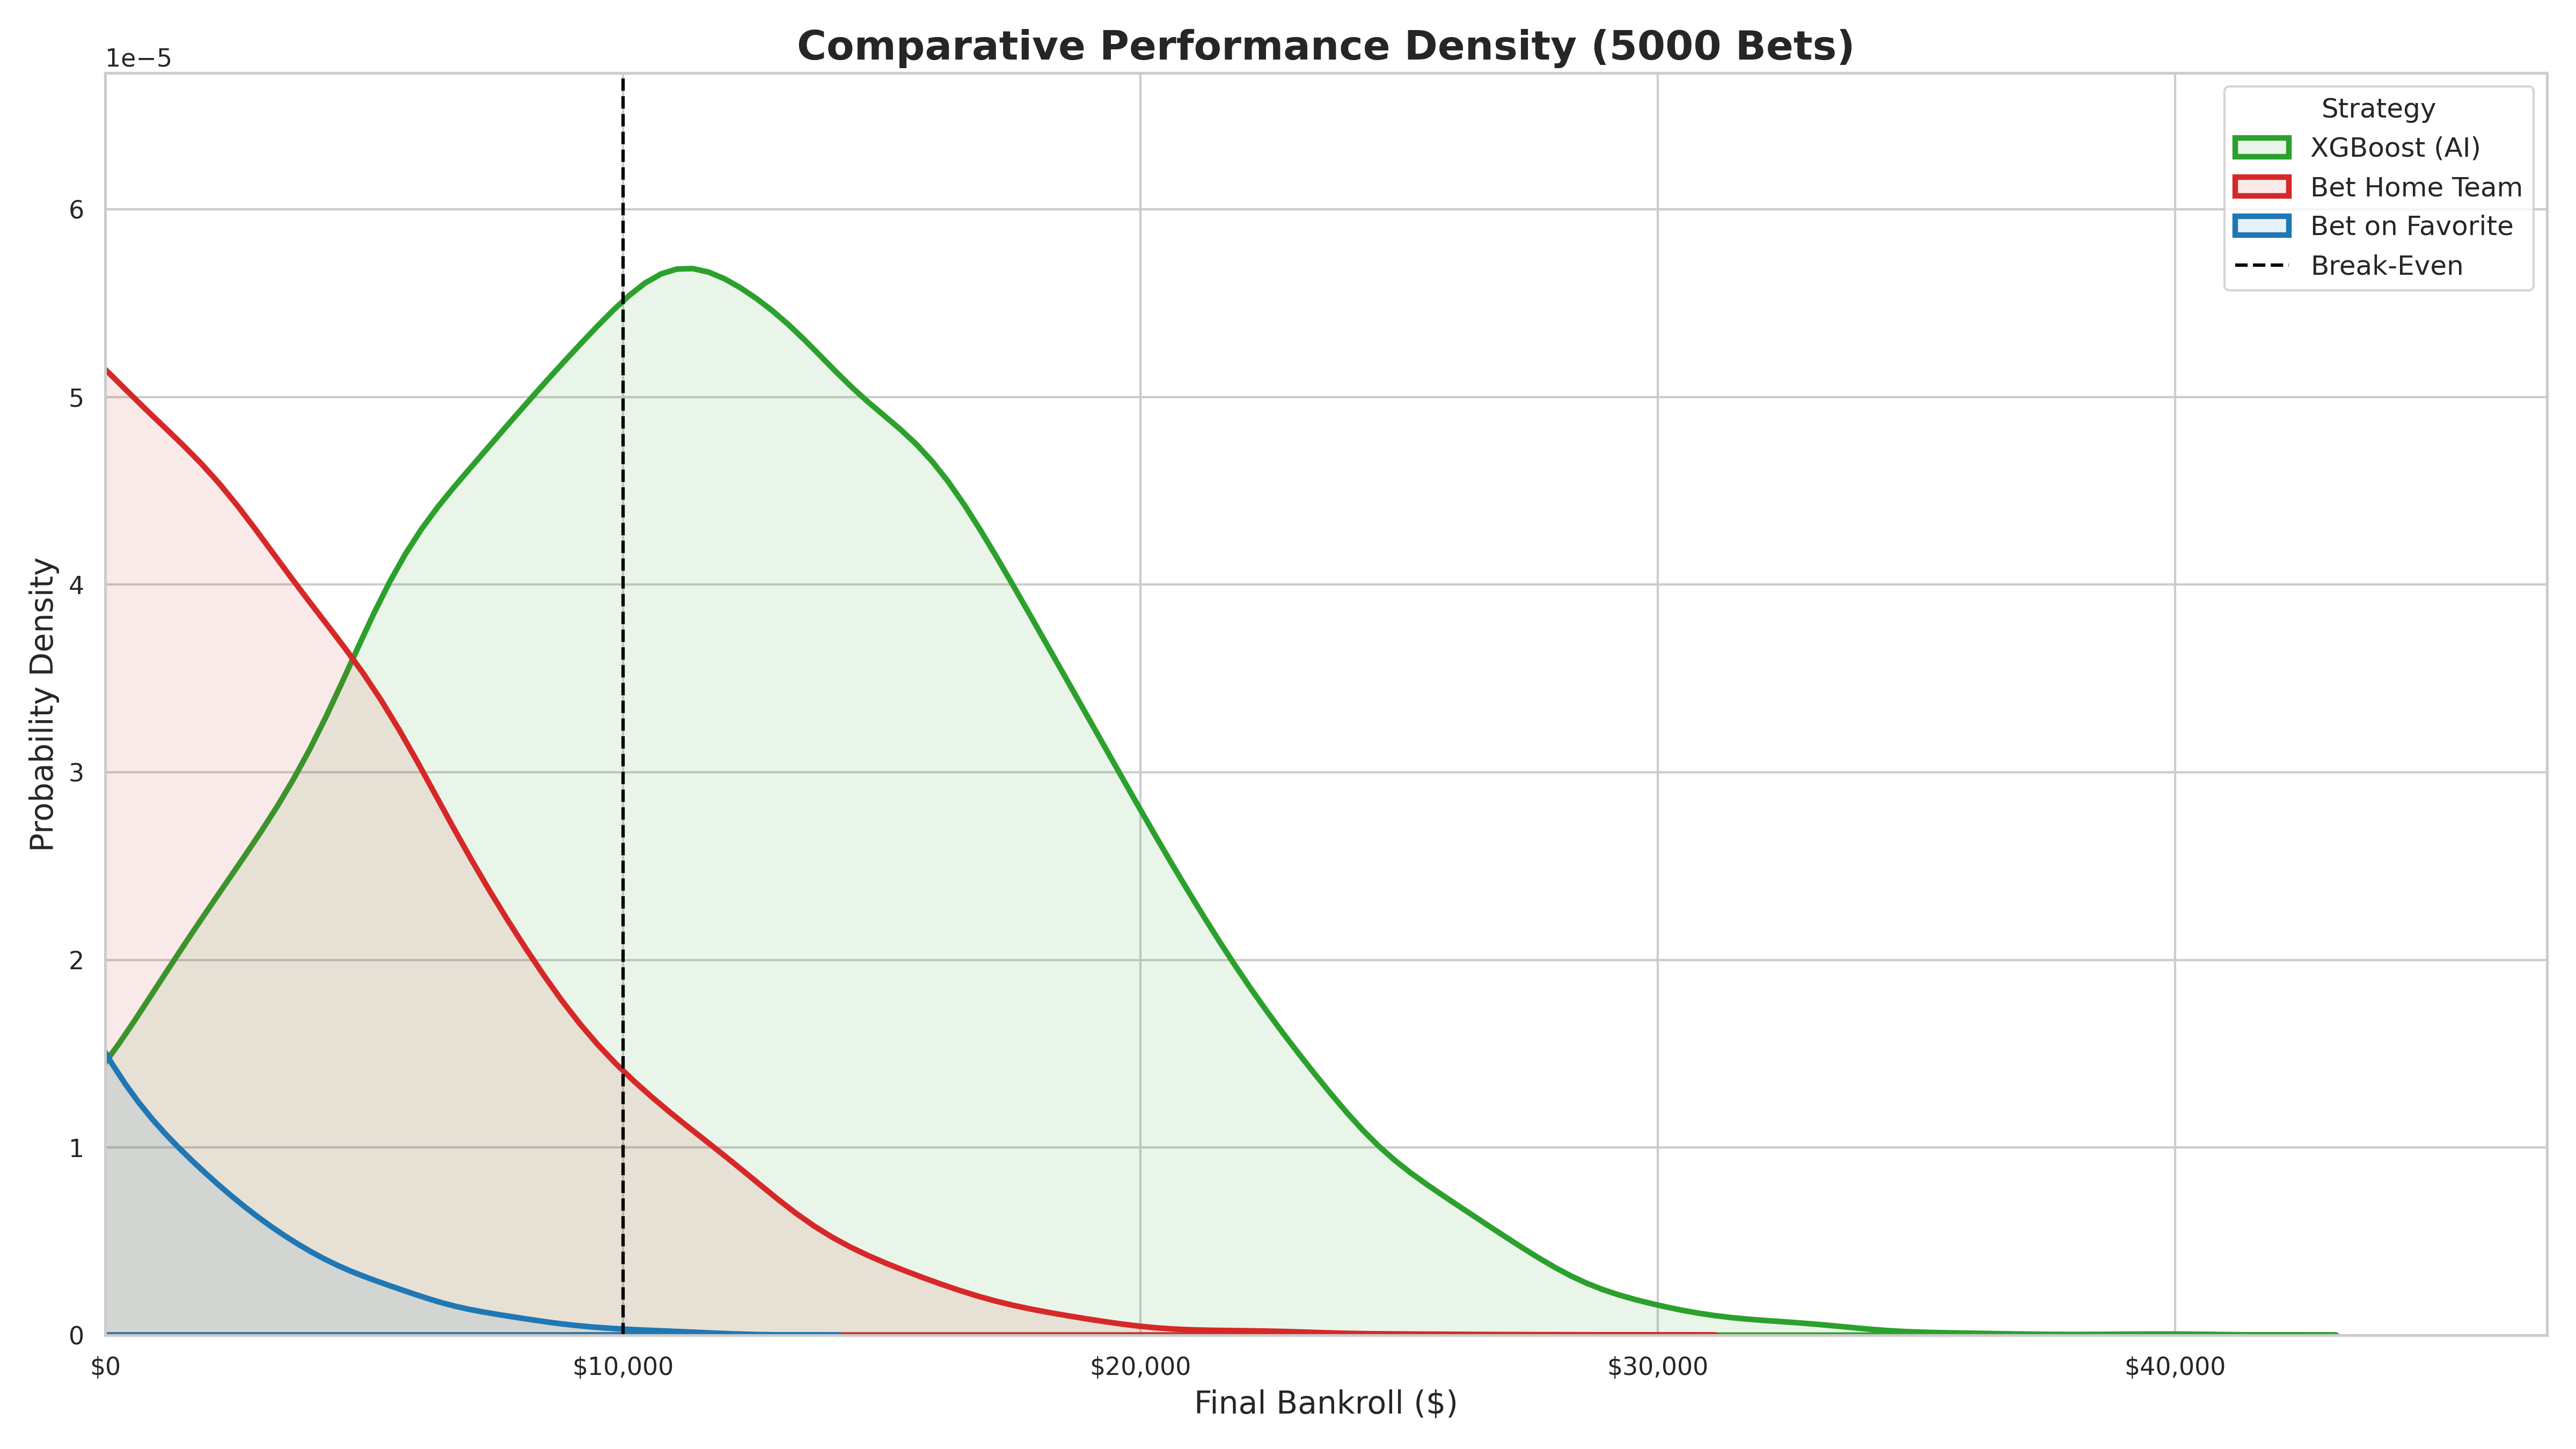
\includegraphics[width=1.0\textwidth]{Fig10.png}
    \caption{Comparative Performance Density. This chart overlays the AI's performance (green) against human strategies. The AI curve is taller and shifted right, meaning it produces consistent, moderate results more often than the volatile human strategies.}
    \label{fig:comparative_kde}
\end{figure}

% --- DISCUSSION ---
\section{Discussion}

Our findings offer a cautionary tale for the application of machine learning in competitive, human-driven markets. The failure of sophisticated models to generate a consistent profit in the modern era (post-2015) without strict calibration is not a failure of the algorithms themselves, but a testament to the efficiency of the market they are trying to beat.

\subsection{The Evolution of the Opponent}
The clear decay in performance over time supports the "Adaptive Market Hypothesis." In 2006, a standard gradient boosting algorithm could likely outpace the human compilers setting the odds. Today, those same bookmakers are almost certainly using similar, if not superior, automated systems, compounded by the financial leveling of the Premier League. We are no longer playing against a human; we are playing against a mirror. The market has effectively "priced in" the very technology we are trying to use against it.

\subsection{The Danger of Metric Fixation}
This study also highlights a flaw in how data scientists typically evaluate models. In a classroom setting, we optimize for Accuracy or AUC (Area Under the Curve). By those standards, our models looked fine—especially Logistic Regression, which correctly predicted outcomes 54.1\% of the time. However, in an applied setting where risk management is key, "Accuracy" is a dangerously misleading metric. 

As demonstrated by the Fractional Kelly simulations, \textbf{Calibration} is the more vital metric. A model that knows it is guessing (and bets small) is infinitely more useful than a model that thinks it is a genius (and bets big). The calibration correction via Isotonic Regression was the singular difference between a bankrupt investment strategy and a profitable one.

\subsection{Alternative Strategies for Mitigation}
While our fundamental models required strict calibration to survive, other approaches exist in the literature. Kaunitz et al. (2017) demonstrated that strategies focusing purely on "consensus odds"—identifying outliers where one bookmaker is slow to update compared to the rest of the market—can still yield profits without analyzing team performance at all \cite{kaunitz2017}. This perfectly aligns with our Ablation Study findings: predicting the \textit{game} is nearly impossible, but predicting \textit{market errors} remains viable. Conversely, Boshnakov et al. (2017) achieved success using bivariate Weibull count models, suggesting that perhaps our fundamental feature set was too simplistic and that highly complex parametric models still hold value \cite{boshnakov2017}.

% --- LIMITATIONS ---
\section{Limitations}

While this study provides robust empirical evidence regarding market efficiency, certain constraints in our scope and methodology must be acknowledged to contextualize the findings.

\subsection{Data Availability and Feature Scope}
Our sports betting analysis relied on a public dataset that, while historically extensive (2000–2021), was limited in feature depth. The dataset contained only match-level statistics and odds. We did not incorporate granular data points such as player-level injuries, lineup changes, or advanced metrics like Expected Goals (xG) simply because reliable historical data for these features was unavailable for the full twenty-year period. It remains an open question whether a model trained on such deep, granular data could uncover inefficiencies that our match-level models missed.

\subsection{Closing Line Rigidity}
Our Walk-Forward validation tested the models against the "Closing Odds"—the final price available before the match starts. The "Closing Line" is statistically proven to be the most accurate version of the market price. In a real-world scenario, professional bettors often target "Opening Odds" (days before the match), attempting to identify mispricing before the market corrects it. By testing against the Closing Line, we effectively forced our AI to beat the market at its strongest point. A model that fails against the Closing Line might still have been profitable against the softer Opening Line, though testing this hypothesis requires data that is rarely publicly available.

\subsection{COVID-19 and Concept Drift}
Our analysis revealed a significant vulnerability in historical machine learning models: susceptibility to sudden, unprecedented environmental changes, known formally as "concept drift." During the 2020 season, matches were played in empty stadiums due to the COVID-19 pandemic. Our descriptive statistics show that the structural home-field advantage plummeted from its historical average of approximately 46.5\% down to 42.5\%. Because our models were strictly trained on 15 years of historical data where home-field advantage was a physical certainty, they failed to adapt. The algorithms continued to aggressively bet on home favorites, resulting in a severe -13.24\% financial drawdown during the 2020 walk-forward fold. This highlights a critical limitation of our methodology: historical ML models inherently struggle to adapt to "Black Swan" events that temporarily break the fundamental rules of the training distribution.

\section{Conclusion}

This study began with a simple question: Can standard machine learning algorithms outsmart a highly efficient prediction market? The answer is a qualified "no," unless they are rigorously calibrated. The reasons for this failure—and the subsequent mathematical cure—reveal a great deal about the state of modern data science.

By benchmarking our models against twenty years of real-world betting data, we established through an Ablation Study that models primarily draw their predictive power from the bookmaker's odds rather than team fundamentals. They successfully identify market consensus, but fail to generate sustainable profits using standard risk-management strategies.

The evidence points to a market that has fundamentally changed. The clear Alpha Decay in performance—triggered by the 2015 Leicester City anomaly and the subsequent influx of television broadcast revenue—confirms that the window for simple algorithmic arbitrage has closed, perfectly aligning with the Adaptive Markets Hypothesis. 

Most importantly, our results highlight a critical blind spot in how predictive models are built and tested. The fact that Logistic Regression achieved the highest accuracy (54.1\%) yet generated the largest financial loss, while a Calibrated Fractional Kelly strategy survived the variance to produce a net profit, proves that \textbf{accuracy is not enough}. In a low-margin, high-risk environment, a lack of self-awareness is mathematically fatal.

Ultimately, this research suggests that in mature, adversarial environments, the challenge is no longer about building more complex models to find better answers. The challenge is building more honest models that know when they are guessing. As markets become more efficient, the most valuable trait in an algorithm is not just its ability to predict the future, but its ability to accurately measure its own doubt.


\section*{Declarations}
\begin{itemize}
    \item \textbf{Funding:} The author did not receive support from any organization for the submitted work. No funding was received to assist with the preparation of this manuscript.
    \item \textbf{Competing Interests:} The author has no relevant financial or non-financial interests to disclose.
    \item \textbf{Author Contributions:} Mostafa Shams is the sole author of this work. He conceived the study, conducted the data analysis, programmed the machine learning models, and wrote the entirety of the manuscript.
    \item \textbf{Data Availability:} All data, code, and statistical reports generated during this study are publicly available for review and replication at: \url{https://github.com/MostafaShams5/Research-Accuracy-Without-Profit}. The primary historical odds dataset is derived from Louis Chen's Kaggle repository (2021).
    \item \textbf{Ethical Approval:} Not applicable. This study relies exclusively on publicly available, anonymized sports data and involves no human or animal participants.
    \item \textbf{AI Assistant Disclosure:} An AI assistant (Antigravity) was used strictly for "AI assisted copy editing" purposes, providing formatting adjustments, grammatical refinement, and structural advice on the LaTeX manuscript. All generative analysis, theoretical framework, and code implementation are the original work of the author, who takes full accountability for the final text.
\end{itemize}

% --- BIBLIOGRAPHY ---
\begin{thebibliography}{99}

\bibitem[Fama(1970)]{fama1970}
Fama, E. F. (1970).
\newblock Efficient capital markets: A review of theory and empirical work.
\newblock \emph{The Journal of Finance}, 25(2), 383--417. \url{https://doi.org/10.2307/2325486}

\bibitem[Sauer(1998)]{sauer1998}
Sauer, R. D. (1998).
\newblock The economics of wagering markets.
\newblock \emph{Journal of Economic Literature}, 36(4), 2021--2064. \url{https://www.jstor.org/stable/2565050}

\bibitem[Levitt(2004)]{levitt2004}
Levitt, S. D. (2004).
\newblock Why are gambling markets organized so differently from financial markets?
\newblock \emph{The Economic Journal}, 114(495), 223--246. \url{https://doi.org/10.1111/j.1468-0297.2004.00206.x}

\bibitem[Griffith(1949)]{griffith1949}
Griffith, R. M. (1949).
\newblock Odds adjustments by American horse-race bettors.
\newblock \emph{American Journal of Psychology}, 62(2), 290--294. \url{https://doi.org/10.2307/1418287}

\bibitem[Newall and Cortis(2021)]{newall2021}
Newall, P. W. S., \& Cortis, D. (2021).
\newblock Are sports bettors biased toward longshots, favorites, or both? A literature review.
\newblock \emph{Risks}, 9(1), 22. \url{https://doi.org/10.3390/risks9010022}

\bibitem[Angelini and De Angelis(2019)]{angelini2019}
Angelini, G., \& De Angelis, L. (2019).
\newblock Efficiency of online football betting markets.
\newblock \emph{International Journal of Forecasting}, 35(2), 712--721. \url{https://doi.org/10.1016/j.ijforecast.2018.10.010}

\bibitem[Dixon and Coles(1997)]{dixon1997}
Dixon, M. J., \& Coles, S. G. (1997).
\newblock Modelling association football scores and inefficiencies in the football betting market.
\newblock \emph{Applied Statistics}, 46(2), 265--280. \url{https://doi.org/10.2307/2985633}

\bibitem[Wheatcroft(2020)]{wheatcroft2019}
Wheatcroft, E. (2020).
\newblock Evaluating the impact of calibration on the profitability of betting strategies.
\newblock \emph{International Journal of Forecasting}, 36(3), 1079--1090. \url{https://doi.org/10.1016/j.ijforecast.2019.11.002}

\bibitem[Guo et al.(2017)]{guo2017}
Guo, C., Pleiss, G., Sun, Y., \& Weinberger, K. Q. (2017).
\newblock On Calibration of Modern Neural Networks.
\newblock \emph{Proceedings of the 34th International Conference on Machine Learning}.

\bibitem[Kelly(1956)]{kelly1956}
Kelly, J. L. (1956).
\newblock A New Interpretation of Information Rate.
\newblock \emph{The Bell System Technical Journal}, 35(4), 917--926. \url{https://doi.org/10.1002/j.1538-7305.1956.tb03809.x}

\bibitem[Walsh and Joshi(2024)]{walsh2024}
Walsh, A., \& Joshi, A. (2024).
\newblock Calibration is all you need: Maximizing utility in sports betting.
\newblock \emph{arXiv preprint arXiv:2401.00000}.

\bibitem[Chen(2021)]{kaggleEPL}
Chen, L. (2021).
\newblock Football Results and Betting Odds Data of EPL. [Data set].
\newblock Kaggle. \url{https://www.kaggle.com/datasets/louischen7/football-results-and-betting-odds-data-of-epl}

\bibitem[Diebold and Mariano(1995)]{diebold1995}
Diebold, F. X., \& Mariano, R. S. (1995).
\newblock Comparing Predictive Accuracy.
\newblock \emph{Journal of Business \& Economic Statistics}, 13(3), 253--263. \url{https://doi.org/10.1080/07350015.1995.10524599}

\bibitem[Baker and McHale(2013)]{baker2013}
Baker, R. D., \& McHale, I. G. (2013).
\newblock A time-varying hazard model for the exact time of goals in football.
\newblock \emph{International Journal of Forecasting}, 29(4), 684--692. \url{https://doi.org/10.1016/j.ijforecast.2012.11.001}

\bibitem[Kaunitz et al.(2017)]{kaunitz2017}
Kaunitz, L., Zhong, S., \& Kreiner, J. (2017).
\newblock Beating the bookies with their own numbers - and how the online sports betting market is rigged.
\newblock \emph{arXiv preprint arXiv:1710.02824}.

\bibitem[Boshnakov et al.(2017)]{boshnakov2017}
Boshnakov, G. N., Kharrat, T., \& McHale, I. G. (2017).
\newblock A bivariate Weibull count model for forecasting association football scores.
\newblock \emph{International Journal of Forecasting}, 33(2), 458--466. \url{https://doi.org/10.1016/j.ijforecast.2016.11.006}

\bibitem[Murphy and Winkler(1987)]{murphy1987}
Murphy, A. H., \& Winkler, R. L. (1987).
\newblock A general framework for forecast verification.
\newblock \emph{Monthly Weather Review}, 115(7), 1330--1338. \url{https://doi.org/10.1175/1520-0493(1987)115<1330:AGFFFV>2.0.CO;2}

\bibitem[MacLean et al.(2011)]{maclean2010}
MacLean, L. C., Thorp, E. O., \& Ziemba, W. T. (2011).
\newblock \emph{The Kelly Capital Growth Investment Criterion: Theory and Practice}.
\newblock World Scientific. \url{https://doi.org/10.1142/7598}

\bibitem[Zadrozny and Elkan(2002)]{zadrozny2002}
Zadrozny, B., \& Elkan, C. (2002).
\newblock Transforming classifier scores into accurate multiclass probability estimates.
\newblock \emph{Proceedings of the eighth ACM SIGKDD international conference on Knowledge discovery and data mining}, 694--699. \url{https://doi.org/10.1145/775047.775151}

\bibitem[Peeters(2011)]{peeters2011}
Peeters, T. (2011).
\newblock Broadcasting rights and competitive balance in European soccer.
\newblock \emph{International Journal of Sport Finance}, 6(1), 23--39.

\bibitem[Lo(2004)]{lo2004}
Lo, A. W. (2004).
\newblock The Adaptive Markets Hypothesis: Market Efficiency from an Evolutionary Perspective.
\newblock \emph{The Journal of Portfolio Management}, 30(5), 15--29. \url{https://doi.org/10.3905/jpm.2004.442611}

\end{thebibliography}

\end{document}
